\documentclass[12pt]{article}
\usepackage[a4paper,margin=2.0cm]{geometry}
\usepackage[T1]{fontenc}
\usepackage{lmodern}
\usepackage{microtype}
\usepackage{amsmath}
\usepackage{booktabs}
\usepackage{array}
\usepackage{longtable}
\usepackage{graphicx}
\usepackage[super,sort&compress]{natbib}
\usepackage[colorlinks=true,allcolors=blue]{hyperref}
\usepackage{xurl}
\usepackage{bookmark}
\usepackage{lineno}
\hypersetup{pdftitle={A reusable solvent-response framework for molecular hydration prediction},
  pdfauthor={Gal Oren, Boris Fain, Michael Levitt},bookmarksopen=true}
\newcommand{\doi}[1]{\href{https://doi.org/#1}{\nolinkurl{https://doi.org/#1}}}
\usepackage{xcolor}
\usepackage{caption}
\usepackage{placeins}
\usepackage{flafter}
\usepackage{enumitem}
\usepackage{tabularx}
\graphicspath{{supplementary/figures/}}
\newcommand{\BenchmarkN}{85}
\newcommand{\ClassicalMAE}{0.785}
\newcommand{\PIMDMAE}{0.205}
\newcommand{\MatchedMAE}{0.303}
\newcommand{\SolvAIMAE}{0.202}
\newcommand{\SolvAIDelta}{\ensuremath{-0.101}}
\newcommand{\SolvAICILow}{\ensuremath{-0.215}}
\newcommand{\SolvAICIHigh}{\ensuremath{-0.020}}
\newcommand{\RepeatMean}{0.207}
\newcommand{\RepeatSD}{0.004}
\newcommand{\MatchedRepeatMean}{0.313}
\newcommand{\NarrowMAE}{0.212}
\newcommand{\NarrowSMDMAE}{0.207}
\newcommand{\ShuffledMAE}{0.306}
\newcommand{\FamilyMAE}{0.468}
\newcommand{\ScaffoldMAE}{0.376}
\newcommand{\ClusterMAE}{0.216}
\newcommand{\NNSeventyMatchedMAE}{0.343}
\newcommand{\NNSeventySolvAIMAE}{0.211}
\newcommand{\FamilyMatchedMAE}{1.262}
\newcommand{\ScaffoldMatchedMAE}{0.728}
\newcommand{\ZeroArrowMatchedMAE}{0.385}
\newcommand{\ZeroArrowMAE}{0.257}
\newcommand{\MolSolvN}{350,359}
\newcommand{\ConfSolvN}{17,829}
\newcommand{\TierAN}{220}
\newcommand{\TierAStructureMAE}{1.532}
\newcommand{\TierASolvAIMAE}{1.153}
\newcommand{\TierADelta}{\ensuremath{-0.379}}
\newcommand{\TierACILow}{\ensuremath{-0.517}}
\newcommand{\TierACIHigh}{\ensuremath{-0.248}}
\newcommand{\TierAStrictN}{97}
\newcommand{\TierAStrictStructureMAE}{2.138}
\newcommand{\TierAStrictSolvAIMAE}{1.536}
\newcommand{\TierAStrictDelta}{\ensuremath{-0.603}}
\newcommand{\TierAStrictCILow}{\ensuremath{-0.863}}
\newcommand{\TierAStrictCIHigh}{\ensuremath{-0.359}}
\newcommand{\WeightOneStructureMAE}{0.310}
\newcommand{\WeightOneSolvAIMAE}{0.206}
\newcommand{\WeightOneDelta}{\ensuremath{-0.103}}
\newcommand{\WeightOneCILow}{\ensuremath{-0.219}}
\newcommand{\WeightOneCIHigh}{\ensuremath{-0.020}}
\newcommand{\WarmSingleSeconds}{15.29}
\newcommand{\BatchSeconds}{15.82}
\newcommand{\BatchPerMoleculeSeconds}{0.494}
\newcommand{\SolvAIReduction}{0.101}

\newcommand{\ComputedOnlyMAE}{\ensuremath{0.234}}
\newcommand{\ComputedOnlyDelta}{\ensuremath{-0.069}}
\newcommand{\ComputedOnlyLow}{\ensuremath{-0.191}}
\newcommand{\ComputedOnlyHigh}{\ensuremath{0.022}}

\captionsetup{font=small,labelfont=bf}
\setlength{\parindent}{1.2em}
\setlength{\parskip}{0pt}
% Full-page figures begin at the top margin rather than being vertically
% centered on a float page.
\makeatletter
\setlength{\@fptop}{0pt}
\setlength{\@fpbot}{0pt plus 1fil}
\makeatother

% Unnumbered journal headings remain unnumbered on the page, but every section
% and subsection is directly navigable in the complete PDF's bookmarks.
\NewCommandCopy{\journalOriginalSection}{\section}
\RenewDocumentCommand{\section}{s o m}{%
  \IfBooleanTF{#1}{\journalOriginalSection*{#3}\addcontentsline{toc}{section}{#3}}%
  {\IfNoValueTF{#2}{\journalOriginalSection{#3}}{\journalOriginalSection[#2]{#3}}}}
\NewCommandCopy{\journalOriginalSubsection}{\subsection}
\RenewDocumentCommand{\subsection}{s o m}{%
  \IfBooleanTF{#1}{\journalOriginalSubsection*{#3}\addcontentsline{toc}{subsection}{#3}}%
  {\IfNoValueTF{#2}{\journalOriginalSubsection{#3}}{\journalOriginalSubsection[#2]{#3}}}}

\title{A reusable solvent-response framework for molecular hydration prediction}
\author{%
Gal Oren$^{*}$, Boris Fain and Michael Levitt$^{*}$\\[0.4em]
\small Stanford University, Stanford, California, USA
}
\date{}


\usepackage{xr-hyper}
\externaldocument[M-]{main}
\begin{document}
% !TEX root = ../main.tex
% Included by main.tex; compile the root document, not this fragment.
\section*{Supplementary Information}
\noindent Supplementary Methods S1--S22; Supplementary Notes S1--S2;
 Supplementary Tables 1--18; Supplementary Figures 1--12; Supplementary Data 1--6.

\section*{Supplementary Methods}

\subsection*{S1. Reference-set processing}

The ARROW reference table was reconstructed from machine-readable project outputs and
contains 85 unique neutral solutes in water at 298 K. One molecule--condition row was
retained for each connectivity. The reference includes experimental hydration free
energy and, where available in the source, uncertainty, classical ARROW, PIMD4 and
PIMD8 values. Molecular names were not used for identity. Canonical isomeric SMILES,
full InChIKey and the first InChIKey block were generated with RDKit 2026.03.5. The
released benchmark table is \texttt{data/benchmark/arrow\_solvation\_master.parquet}.

The reconstructed ARROW/PIMD8 MAE is 0.204836 kcal mol$^{-1}$ and the classical
ARROW MAE is 0.784648 kcal mol$^{-1}$. These values are direct errors against the same
experimental column used for SolvAI evaluation; neither simulation value is an input
to the final model.

\subsection*{S2. Public endpoint labels}

The endpoint-label catalog initially contained 5,075 benchmark-disjoint
connectivities. A frozen source-quality rule retained all 1,147 rows from an earlier
FreeSolv/CombiSolv-Exp merge and 133 additional SoluteML dGsolvDB3 rows supported by
at least two source measurements, giving 1,280 public labels. Duplicate structures
were resolved at the connectivity level before this rule was applied. The source
composition is listed in Supplementary Table~3. The raw merged tables are not
redistributed where source terms are not explicit; URLs, versions, hashes and
reconstruction commands are given in \texttt{repro/DATA\_PROVENANCE.md}.
CombiSolv-Exp originates from the collection of Vermeire and Green;\cite{combisolv2021}
the version used here was downloaded from the SolvBERT repository mirror.\cite{combisolvexp2022}

For a random outer fold, these 1,280 rows were combined with the available ARROW
outer-training molecules. Public rows received sample weight 1 and ARROW
outer-training rows weight 3. The experimental value of an outer-test molecule was
never used. In the zero-ARROW transfer experiment, only the 1,280 public labels
were fitted and all 85 ARROW molecules were evaluated.

The weight of 3 was part of the prospective confirmatory protocol rather than a
post-result choice. A separately prespecified one-factor sensitivity changed only the
available ARROW outer-training weight to 1. Under this setting, matched structure-only
and response-augmented ExtraTrees MAEs are 0.30977 and 0.20642 kcal mol$^{-1}$, respectively; the paired
change is $-0.10335$ kcal mol$^{-1}$ (95\% interval, $-0.21883$ to $-0.01995$).

\subsection*{S3. Response-source processing}

\paragraph{CombiSolv-QM.}
The water subset was deduplicated by solute connectivity and expressed in kcal
mol$^{-1}$. After the original exact-connectivity exclusion, 3,961 structures were
available. Conservative canonical-tautomer comparison found two additional
benchmark equivalents; the confirmatory surrogate therefore used 3,959 rows.

\paragraph{SoluteML Abraham parameters.}
Five Abraham solute axes (E, S, A, B and L) were predicted from 8,098
benchmark-disjoint structures. These coordinates respectively describe excess molar
refraction, dipolarity/polarizability, hydrogen-bond acidity, hydrogen-bond basicity
and gas-to-hexadecane partition response. No standardized benchmark equivalent was
found in the audited source.

\paragraph{OpenFF explicit-water response.}
The source contains 520 benchmark-disjoint absolute solvation-free-energy records
from an OpenFF 2.3.0/NAGL/TIP3P protocol with 14 alchemical states. The records
come from the Open Free Energy (OpenFE) alchemical benchmark resources release,\cite{openffdata2026}
using version 2.3.0 of the OpenFF Sage force-field family.\cite{openffsage2023} Separate
ExtraTrees models predicted calculated hydration free energy and its experimental
residual, defined as experimental hydration free energy minus the original
calculated hydration free energy, not minus a surrogate prediction. Their sum
is the retained corrected OpenFF coordinate.

\paragraph{GBn2 implicit response.}
The source contains 550 benchmark-disjoint GBn2 hydration calculations. GBn2 is the
generalized Born model of Nguyen, Roe and Simmerling;\cite{gbn22013} the calculation
records were obtained from the dataset released by Katzberger and Riniker.\cite{gnnis2024} Separate
ExtraTrees models predicted the calculated value and its experimental residual. The
sum is the retained corrected implicit-solvent coordinate. Its residual target
uses the same experiment-minus-original-calculation definition.

\paragraph{MolSolv SMD(water).}
The source archive contains 1,729,545 M06-2X/6-31G* SMD calculations. The frozen
selection retained all eligible neutral structures with at most 10 heavy atoms and a
deterministic one-in-eight sample for structures with 11--18 heavy atoms. After
deduplication and exact-connectivity filtering, 350,391 rows remained. Canonical
tautomer standardization identified 32 additional benchmark-equivalent records. The
confirmatory model used 350,359 rows while keeping every retained molecule in its
original source split.

\paragraph{ConfSolv H$_2$O.}
The archive contains 5,392,567 H$_2$O conformer records for 43,693 solutes. We
converted kJ mol$^{-1}$ to kcal mol$^{-1}$ and aggregated conformers into gas,
water and hydration conformer corrections together with water-response
distribution summaries. The broader quality filter produced 39,878 neutral
connectivities. The selected surrogate target set had 17,851 rows with complete
features and admissible energy range; fragment-parent, uncharging and tautomer
standardization removed 22 additional benchmark-equivalent records, leaving 17,829.

\subsection*{S4. The 15 response descriptors}

Supplementary Table~1 defines every retained coordinate. At inference, the table's
``surrogate'' column is the calculation that runs; the expensive source method does
not. The final vector contains one CombiSolv-QM response, five Abraham axes, one
corrected OpenFF response, one corrected GBn2 response, one SMD(water) response and
six ConfSolv summaries, for 15 coordinates in total.

Richer CombiSolv, OpenFF, GBn2 and ConfSolv targets were
available and were evaluated during model development. Only the listed coordinates
belong to the released stack. In particular, no PIMD2, PIMD4, PIMD8,
$\mathrm{d}H/\mathrm{d}\lambda$ or NQE coordinate is present.

\subsection*{S5. Surrogate models}

The CombiSolv-QM and MolSolv targets were fitted with Chemprop 2.2.4
directed-message-passing models initialized from CheMeleon. Both used a two-layer
feed-forward head of width 256, dropout 0.1, initial/maximum/final learning rates of
$3\times10^{-5}$, $10^{-4}$ and $10^{-5}$, and PyTorch seed 20260826. CombiSolv-QM
used RDKit two-dimensional descriptors, batch size 64, a 30-epoch cap and patience 7; MolSolv used the
molecular graph, batch size 256, a 25-epoch cap and patience 6. The original frozen
train/validation/test memberships were 80/10/10\% for CombiSolv-QM and 90/5/5\% for
MolSolv. Standardized equivalents were removed from their existing split rather than
resplitting the remaining source.

Abraham, OpenFF and GBn2 targets used ExtraTrees regressors on the same 2,265
structure features used by the endpoint. The selected leaf sizes and target-level
OOF errors are recorded in the source metadata. ConfSolv used 217 RDKit descriptors
and the 256 highest-variance Morgan bits. Each target was fitted with a LightGBM
L1-regression model with 450 estimators, learning rate 0.04, 31 leaves, minimum child
size 20, row subsampling 0.8, column subsampling 0.55 and $L_2$ regularization 0.1.
Target-specific seeds were 20260826 plus the target index for validation and 1000
plus that index for the all-retained-source fit.

For OpenFF and GBn2, source records were matched to public endpoint candidates by
connectivity. Public molecules represented in a source table received predictions
from five-fold source-level out-of-fold fits for each physical and residual target;
other public molecules and ARROW molecules received the corresponding full-source
model predictions. Minimum leaf size was selected from 1, 2 and 3 using those same
source folds. Thus the recorded source OOF errors are selection scores, not nested
unbiased validation estimates. These source folds were fixed independently of the
later endpoint partitions; they were not rebuilt for chemical- or size-held-out
endpoint fits. Source-OOF feature generation therefore differs from excluding an
entire downstream holdout from source supervision. The source-preparation scripts
are archived under \texttt{repro/response\_sources/}.

The recorded OpenFF physical/residual OOF MAEs are 0.617/0.531 kcal mol$^{-1}$;
the corresponding GBn2 values are 0.669/0.626. These are errors of separate source
components, not of their corrected sum. The standardized-exclusion ConfSolv
validation contains 1,785 molecules and gives MAEs of 0.248, 0.267, 0.354, 0.448,
0.688 and 0.450 kcal mol$^{-1}$ for coordinates 10--15 in Supplementary Table~1.
These heterogeneous source checks do not form a common independent fidelity
benchmark for all 15 coordinates; the endpoint comparisons assess their predictive
utility rather than presuming uniform recovery accuracy.

\subsection*{S6. Matched ExtraTrees implementation}

The molecular representation comprises a 2,048-bit radius-2 Morgan fingerprint and
217 RDKit two-dimensional descriptors. The confirmatory endpoint appends the 15 response descriptors,
giving 2,280 columns. A median imputer is fitted on each training partition and adds
missingness indicators only where required. Each of three
\texttt{ExtraTreesRegressor} models uses 360 trees, squared-error splitting,
\texttt{max\_features}=0.7, \texttt{min\_samples\_leaf}=2,
\texttt{min\_samples\_split}=2, unlimited depth and no bootstrap; seeds are 11, 29
and 47. Predictions are averaged. The matched structural model removes only the 15
response columns.

After all evaluation was frozen, the release artifact was refitted on the 1,280
public labels and all 85 ARROW labels using the same weights and configuration.
That refit supplies deployment predictions and the endpoint-disjoint external
evaluation. Reported ARROW held-out scores use only the appropriate fold-specific
fits.

\subsection*{S7. Validation partitions}

The fixed primary result uses the released \texttt{fold\_random} assignment. Five
complete repeated five-fold partitions use shuffled K-fold seeds 314159, 271828,
161803, 141421 and 173205. All comparisons use the same fold, training rows and model
seeds within a partition.

For functional-family separation, SMARTS rules were applied in the precedence order
carboxylic acid, amide, ester, aldehyde, ketone, alcohol/phenol, ether, amine, thiol,
sulfide/disulfide, aromatic heterocycle, carbocyclic aromatic, alkene/diene,
saturated hydrocarbon and other. A test-fold family was removed from both public and
ARROW endpoint training rows. Bemis--Murcko scaffold separation used canonical
isomeric scaffold SMILES; acyclic molecules were keyed by primary family. Molecular
clusters were constructed once on the combined endpoint pool with Taylor--Butina
clustering at Morgan Tanimoto similarity 0.70. Nearest-neighbor analyses excluded
training rows at similarity thresholds 0.50, 0.60, 0.70 and 0.80 to any outer-test
molecule.

\subsection*{S8. Shuffled-descriptor control}

All 15 response columns were permuted together to preserve their joint distribution.
For each outer fold, public, ARROW outer-training and ARROW outer-test response rows
were permuted separately. The experimental target was never used to define a
permutation. Five base seeds (88001--88005) were used for the fixed partition and
each repeated partition. This control changes molecule--response alignment while
retaining feature count, response marginal distributions and inter-descriptor
correlations.

\subsection*{S9. Statistical analysis}

MAE is primary. RMSE, median absolute error and the fraction of molecules
improved are secondary. Paired candidate-minus-reference differences were resampled
at molecule level 100,000 times with seed 20260828. The 2.5th and 97.5th
percentiles define the reported intervals. For the five repeated partitions, each
molecule's absolute error was first averaged over partitions before paired
resampling. The prespecified protocol defined a positive comparison as a complete interval
below zero. We report all prespecified comparisons without multiplicity adjustment
and do not treat the panel as a single confirmatory hypothesis test. The protocol
and its implementation amendments are archived in Git at
\nolinkurl{release/CONFIRMATORY_FREEZE.md}; the amendments preceded the corrected runs.
For the additional molecular-model comparisons, the released
\nolinkurl{results/endpoint_models_20261006/corrected_original_metrics.csv} also provides the coefficient of
determination ($R^2$) for each model and cohort.

\subsection*{S10. External validation}

The original 221-molecule cohort was frozen for a separate solvation-model validation
study before that study's model predictions. It was derived from type-M original-measurement
records in Sander's Henry-law compilation v5.0.0. Intrinsic pure-water
$H_s^{cp}$ values (aqueous concentration divided by gas partial pressure),
normalized to 298.15 K, were converted as
$K_c=H_s^{cp}RT$ and $\Delta G_{\rm hyd}=-RT\ln K_c$, where $K_c$ is the
dimensionless aqueous-to-gas concentration ratio. This produces the same 1 M
gas-to-1 M aqueous standard-state convention used for the endpoint. The source values
are printed to two significant figures.

SolvAI qualification was performed without reading SolvAI predictions or errors. All
221 rows passed the connected, neutral, supported-element and target-compatibility
rules. One candidate was excluded because that study's registry audit had documented a
definite conflict between its registry name/CAS and supplied InChIKey structure. The
remaining 220 molecules had no exact, fragment-parent, uncharged-parent or
canonical-tautomer equivalent among the 1,280 public or 85 ARROW endpoint labels.
Of these, 123 occurred in at least one supervised response-source table and 97 were
absent from all six. The latter define the strict response-source-disjoint subset.
The cohort hashes, all exclusions and all response-source matches were recorded in Git before
endpoint evaluation.

Both endpoint models were then fitted deployment-style on the same 1,280 public
plus 85 ARROW labels with weights 1 and 3. They used the same descriptors, imputation,
three 360-tree ensembles and seeds; only the 15 response columns differed. No external-cohort
label entered fitting or selection. On N=220, structure-only and response-augmented
ExtraTrees MAEs were
1.53165 and 1.15255 kcal mol$^{-1}$ (paired change $-0.37909$; 95\% interval,
$-0.51692$ to $-0.24817$). On strict N=97, the corresponding values were 2.13830 and
1.53560 kcal mol$^{-1}$ (paired change $-0.60271$; interval, $-0.86277$ to $-0.35858$).
The absolute errors delimit applicability and are not presented as PIMD8-level
performance outside ARROW-85.

\subsection*{S11. Lambda-response probes}

Short PIMD2 response fingerprints were available at $\lambda=0.1$, 0.5 and 0.9 for
72, 74 and 73 molecules, respectively; 72 had complete three-point curves. The
targets were the total solute--solvent $\mathrm{d}H/\mathrm{d}\lambda$ and its
electrostatic and van der Waals components. A zero-valued polarization field was not
interpreted. Structure-only heads were evaluated by OOF prediction, and their
outputs were added to the fixed SMD(water) plus ConfSolv response baseline for
this exploratory ablation (MAE 0.1959 kcal mol$^{-1}$). A separate direct-integration experiment used the predicted three-point
curve with an affine calibration fitted inside each outer training fold. These
targets were evaluated as candidate supervision and were not retained.

\subsection*{S12. Artifact verification}

The public API accepts one or more SMILES strings. RDKit parses each input and emits
canonical isomeric SMILES before feature generation. It does not standardize a query
across tautomers, protonation states or salt forms. The runtime computes descriptors,
evaluates the two D-MPNNs and four tree-artifact families, and
passes the resulting 2,280-vector to three endpoint regressors. The artifact audit
checks file hashes, feature count and names, software versions and two smoke
predictions. It rejects features containing experimental target, PIMD, trajectory,
probe, fold or scaffold information. The standardized-exclusion surrogate refit is
identified in the model card and manifest. The ensemble spread is returned for
diagnosis but is not a calibrated per-query applicability or reliability score.

\subsection*{S13. Runtime benchmarking}

Runtime was measured end to end from input SMILES to prediction on the released
artifact. The host used an Intel Core i7-4930K CPU; the installed NVIDIA RTX 3090 was
not used for inference. Cold single-molecule latency, five warm single-molecule
runs, three batch-32 runs and peak resident memory were recorded. Chemprop predictor
startup dominates single-molecule latency. These measurements describe the released
implementation, not the irreducible model cost. The ARROW/PIMD8 comparison uses the
published 15-window protocol and is kept separate from same-host inference timing.

\subsection*{S14. Additional molecular-model comparisons}

The additional molecular-model comparison uses the existing 1,280 public endpoint labels,
85 ARROW labels and 220 external test molecules. The protocol was fixed before the
new fits, but these are retrospective comparisons on already examined datasets.
The original fixed five-fold ARROW assignments are retained. For the external test,
all 1,365 endpoint labels are used; the 97-molecule source-disjoint subset is fixed
before these comparisons and is not a separate fit. Public labels have weight 1 and
ARROW training labels weight 3 throughout. The wider optimization study in S18
is a separate comparison, not a reinterpretation of these fixed 80-epoch fits.

The scratch D-MPNN has message dimension 300, three message-passing steps, mean
aggregation, a regression head with two hidden layers of 300 units and dropout 0.1. The CheMeleon
model initializes message passing from the published
\texttt{chemeleon\_mp.pt} weights, retains their encoder configuration and fine-tunes
that encoder; it uses the same regression-head dimensions and dropout.
Both optimize squared error using Adam and batch size 64, with constant learning
rates $3\times10^{-4}$ and $10^{-4}$, respectively. Target scaling is fitted on the
training subset only. For each outer partition and model seed, a deterministic 15\%
of each source is held out internally (split seed $20261002+\text{model seed}$).
The epoch with lowest unweighted validation MAE is selected, with a cap of 80 epochs
and patience 12. A model reinitialized from the same random or CheMeleon starting
weights is then fitted on all outer-training
labels for that many epochs, using a newly fitted training scaler. This restores
the inner-validation molecules to the final training pool without exposing the
outer test labels. Predictions from seeds 11, 29 and 47 are averaged. Every selected
epoch, validation trace, training identity and held-out identity is retained.
Supplementary Fig.~6 shows the order of inner selection, fresh refitting and
held-out scoring.

MoLFormer uses the published
\nolinkurl{ibm-research/MoLFormer-XL-both-10pct} model at revision
\nolinkurl{7b12d946c181a37f6012b9dc3b002275de070314}. The 768-dimensional representation
is the attention-mask mean of the last hidden state, with maximum sequence length
256. Uni-Mol uses its 512-dimensional molecular representation from the
\texttt{mol\_pre\_all\_h\_220816} checkpoint, including hydrogens. Its RDKit
conformer generator uses seed 42. MoLFormer uses the corrected deterministic
representations described in S19; Uni-Mol reuses its original label-free cache,
with missing structures encoded by the same pipeline. Three of the 353
structures absent from the original Uni-Mol embedding cache used the package's two-dimensional fallback after three-dimensional
embedding failed; they are retained rather than excluded by prediction quality.
Both pretrained representations are frozen during endpoint fitting. Molecular
membership in their original pretraining datasets is not audited here.

For each pretrained representation, we fit the same three 360-tree ExtraTrees
regressors on structural features plus that representation, then repeat with the
15 SolvAI response descriptors added. Imputation is fitted inside each training
partition. All families, both feature conditions and all seeds are retained in the
report. The comparison is limited to these fixed training configurations; it is
not an exhaustive hyperparameter optimization or a claim to the best achievable
performance of an architecture. Code and hashed inputs are provided with
\texttt{scripts/run\_journal\_baselines.py}; independent aggregation is provided
with \texttt{scripts/summarize\_journal\_baselines.py}.

\subsection*{S15. Conformational meaning of the response targets}

The experimental endpoint is the equilibrium hydration free energy of a molecular
species. It does not assign a separate target to each geometry of that species.
The ConfSolv H$_2$O subset supplies conformer-resolved gas, water and solvation free energies,
which are aggregated before surrogate training. For gas or water conformer
energies $G_i$, define $g_i=G_i-\min_j G_j$. The conformer correction is
$C=-RT\ln\sum_i\exp(-g_i/RT)$. Two response descriptors are the gas and water
corrections. The third is the difference between the ensemble hydration estimate
and the solvation energy of the lowest-gas-energy conformer. The remaining three
are the population standard deviation of conformer solvation energies and the
arithmetic mean and population standard deviation of
$g_i^{\rm water}-g_i^{\rm gas}$. Source energies are converted from kJ mol$^{-1}$
to kcal mol$^{-1}$. These six summaries characterize the supplied conformer set;
they do not establish complete conformational sampling or provide a geometry-specific
prediction at inference.
Supplementary Fig.~7 illustrates these six summaries and the distinction between
individual conformers and the molecular equilibrium endpoint.

\subsection*{S16. Error as a function of chemical similarity}

For each external molecule, we use the maximum Tanimoto similarity of its
radius-2, 2,048-bit Morgan fingerprint to any of the 1,365 endpoint-training
molecules. Fixed descriptive bins are $[0,0.3)$, $[0.3,0.5)$, $[0.5,0.7)$ and
$[0.7,1]$. We report counts, MAEs and paired differences within each occupied bin.
These are descriptive strata of an existing cohort, not an independently calibrated
applicability-domain threshold. In particular, similarity to endpoint training and
membership in a response-source dataset are different quantities. The exact
molecule-level similarities, predictions and bootstrap intervals are supplied in
\texttt{results/journal\_20261002/}.

\subsection*{S17. Computation-only response control}

A separate source-composition analysis combines ten descriptors derived
solely from computed source targets: COSMOtherm water free energy, uncorrected OpenFF
and GBn2 free energies, SMD(water), and the six ConfSolv summaries. It excludes all
five empirical Abraham parameters and both experimental residual corrections.
The ten descriptors are added to the same 2,265 structural features, with unchanged
five-fold ARROW evaluation, endpoint labels, sample weights, trees and three seeds.
The comparison was specified before fitting this additional control. It measures
whether computed-source descriptors alone improve this learner; it is distinct from
the original three-descriptor computation-core ablation. After the ARROW comparison,
we specified an extension of the same fixed ten-descriptor model to the external
cohort. The OpenFF and GBn2 components are recovered directly from the original
packaged surrogates. Before fitting, their corrected sums must reproduce the frozen
external response cache to within $10^{-10}$ kcal mol$^{-1}$. All other response
descriptors come from that cache. The external fit uses all 1,365 endpoint labels
with the original weights and seeds. Both stages, exact predictions and input hashes
are retained; the extension is explicitly retrospective.

\subsection*{S18. Endpoint architecture and optimization study}

The study reuses the 1,280 public labels, 85 ARROW labels, 220 external identities
and original five-fold ARROW assignments. Source-surrogate weights, targets and
experimental labels are unchanged. It is retrospective, with adaptive development
before a final selection lock; it is not a new prospective validation. Final outer
predictions are made only after training-side selection is complete. The common
selection score averages public-source and ARROW-source validation MAE equally.
Three random inner splits each hold out 15\% of each eligible source, using seeds
$640601+j$ for $j=0,1,2$. Public training rows have loss weight 1 and ARROW rows
weight 3. No external label participates in these fits or inner decisions.

The initial 52-candidate list covers residual MLPs, dual-branch networks,
ridge-plus-neural residuals, pretrained-encoding heads and directed message passing.
Tabular residual blocks apply layer normalization, two linear transforms with GELU
activation and dropout, then add an identity skip. The dual architecture keeps a
separate 32-unit response branch before concatenating it with the structural branch.
The ridge model fits a training-only linear baseline with regularization 10 to the
scaled RDKit and response columns, then trains a residual network on the remaining
target. This is not a ridge model on seven selected responses with a tree residual.
The graph variants use Chemprop bond message passing with either summed and mean
atom embeddings plus atom count, or summed learned atomic outputs plus a global
correction. These readouts carry size information but do not impose exact additivity
of the full free-energy predictor. Frozen-encoder neural heads use separate
structure/encoding and response branches.

Candidate configurations vary widths 32--256, depth, dropout 0--0.2, learning rates
from $3\times10^{-4}$ to $3\times10^{-3}$, weight decay, squared or Huber loss,
and plateau-reduced or cosine schedules. AdamW and batch size 128 are used.
Ordinary neural fits have a 600-epoch cap. Median imputation, constant-column
removal and numerical scaling are fitted inside each training split; response
columns are retained even if constant. Binary Morgan bits remain unscaled.
The skewed Ipc descriptor is transformed by $\log(1+\max(\mathrm{Ipc},0))$ or
removed; BertzCT and Kappa1--3 use signed-log transforms. Physical counts, mass
and surface descriptors are not clipped to the training range. Count-based
fingerprints and later raw-count, log-count and no-fingerprint variants test whether
loss of multiplicity in binary Morgan features limits size response.

Each candidate is screened on split 0 at seed 11. The best two per family proceed
to three splits and seeds 11/29. The family winner is challenged with a 1,200-epoch
cosine schedule on the same three splits at seed 47, against its ordinary schedule.
The longer schedule is retained only if mean validation MAE decreases by more than
0.005 kcal mol$^{-1}$ and at least two of three pairs improve. A retained long
schedule is completed at seeds 11/29, giving nine inner fits. Thus this challenge
changes both duration and learning-rate trajectory, not duration alone. Fresh
outer fits use the median selected epoch and the inner-derived schedule. A width
boundary challenge expands selected 256-unit models to 512 units when a family
selected the upper width in at least four of six partitions; graph message dimension
is expanded as well. The same paired improvement rule determines retention.

TabM adds 12 configurations spanning three fingerprint treatments and four width,
depth, dropout and numerical-embedding settings. Each model uses 32 parameter-sharing
ensemble members; their mean is the prediction.\cite{tabm2025} The study uses TabM
0.0.3 and rtdl-num-embeddings 0.0.12. Representation refinements and the width
extension are retained as explicit selection variants, not relabelled as separate
architectures. Nine of 24 width challenges passed to nine-repeat completion.
All 81 retained wider-fit optima occur before 95\% of their training horizon.
Longer schedules were selected in all six corrected-MoLFormer partitions, five
dual and TabM partitions, three graph partitions, and two residual-MLP and ridge
partitions. Supplementary Fig.~12 shows the paired duration and width diagnostics.

The search contains 1,812 inner evaluation records, including 174 TabPFN context
evaluations. Gradient-based runs total 1,018,212 epochs; TabPFN's 2,112 internal
ensemble passes are not gradient epochs. Summed fitting time is 45.06 hours across
overlapping workers, not elapsed time or GPU-hours. The defined search and boundary
checks completed, but do not exhaust all architectures, regularization choices or
training-data interventions. Full candidate lists and per-partition decisions are
in Supplementary Data~6. Final comparisons retain every family, not only the global
selector. Matched no-response models inherit the response model's recipe, so the
comparison does not estimate each structural-only architecture's best achievable error.

\subsection*{S19. Pretrained representations and TabPFN configuration}

The earlier MoLFormer cache used evaluation mode without enabling the model's
\nolinkurl{deterministic_eval} option. Stochastic attention projections remained
active. All 1,585 study representations and 56 stress-series representations were
therefore regenerated from the same checkpoint with both settings enabled, and
all valid MoLFormer endpoint comparisons were refitted. Identical repeated encoding
gave zero change; changes in query order and batching produced representation
differences below $3\times10^{-5}$. Fresh encoding through endpoint prediction
agreed within $4.9\times10^{-6}$ kcal mol$^{-1}$. Corrected fixed-tree results
replace the earlier cache-based values in Fig.~\ref{M-fig:modern} and Supplementary Tables~11--12.
Legacy stochastic-cache branches remain labelled in the released diagnostic data
and are excluded from valid-model selection and the manuscript's performance
comparisons. Uni-Mol's conformer pipeline and the packaged ExtraTrees endpoint are
unaffected. Original encoder pretraining membership remains unaudited.

TabPFN-3.5 uses \texttt{tabpfn} 9.1.0 and full/Fast checkpoints from revision
\nolinkurl{06bf2ba35c80a92a3b9abb436b99cf49e7a0365e} of
\nolinkurl{Prior-Labs/tabpfn_3_5}.\cite{tabpfn35} Checkpoint SHA-256 values are
recorded in Supplementary Data~6. This specific software release is distinguished
from the earlier tabular foundation-model paper.\cite{tabpfn2025} We use its
pretrained weights without fine-tuning. Inputs retain training-fitted native
preprocessing, including feature subsampling/ranking and target transformations.
The use of a transformer endpoint therefore does not mean that all preprocessing
or the six source-surrogate families are neural.

Eight candidates combine full/Fast weights with four recipes: RDKit plus binary
Morgan bits; RDKit plus raw Morgan counts; RDKit alone; or RDKit plus the corrected
MoLFormer representation. Each has the 15 responses in its full condition.
The best two screen candidates receive repeated inner evaluation. Training-side
challenges compare one versus three copies of each eligible ARROW context row,
and eight versus 32 ensemble passes, using the same greater-than-0.005 and
two-of-three improvement rule. Context repetition occurs after splitting and
does not create new independent observations or equal weighted gradient fitting.
All selected recipes use the full checkpoint and three ARROW copies. The selected
ARROW folds 0--4 use respectively raw counts/8 passes, no fingerprint/32,
no fingerprint/8, raw counts/32, and MoLFormer without fingerprint/8. The external
fit uses MoLFormer without fingerprint and eight passes. These are a per-partition
selection policy, not one identical input recipe across folds.

The comprehensive policy selects the eligible option with lowest repeated inner
score independently in each partition. It selects TabPFN in all six partitions.
Five-seed final predictions use seeds 11, 29, 47, 71 and 101; controls remove only
the responses. Common-three-seed means address the unequal ensemble size relative
to the three-seed ExtraTrees fits. Every fitted-state replay and final identity/label
audit passed. Licensed TabPFN weights and fitted contexts are retained privately;
contexts embed training labels and are not public model-weight substitutes.

\subsection*{S20. Size holdout, homologue series and label influence}

The size split ranks molecules by descending heavy-atom count within public and
ARROW sources, breaking ties by identity. The largest 15\% comprise 192 public
and 13 ARROW molecules, leaving 1,160 training rows. Training heavy-atom counts
range from 0 to 17 and holdout counts from 8 to 37; 188 holdout molecules exceed
the global training maximum. Models use their locked external-fit recipes and
three fresh seeds. ExtraTrees is refitted on these 1,160 rows rather than evaluated
using release weights that have seen the held-out labels. No size score affects
selection. Since the held-out labels participated in earlier random-fold
development, intervals describe this exploratory split, not prospective selection-free
performance on new molecules. Supplementary Table~15 gives all valid family results.
The 13 ARROW molecules retain their original exclusion from supervised source
tables. No analogous source-disjoint guarantee is made for the 192 public molecules:
source models and source-OOF features remain fixed, with no size-specific source
refitting or exposure audit. Accordingly, this is a conditional endpoint comparison,
not a validation of fully source-unseen size extrapolation.

The unlabelled grid contains linear C1--C30 alkanes and Ac-(Gly)$_n$-NHMe and
Ac-(Ala)$_n$-NHMe for $n=0,\ldots,12$. The two zero-residue rows represent the
same N-methylacetamide molecule, so 56 rows are not 56 unique structures. All
positive-length peptides are absent from endpoint training; N-methylacetamide is
present. The longest glycine and alanine examples contain 53 and 65 heavy atoms,
respectively, beyond the maximum 37 in the original training pool. Binary Morgan
fingerprints are identical across $n=2,\ldots,12$ within either peptide family and
across C7--C30 alkanes. Count fingerprints, RDKit descriptors and some predicted
responses still change, so the entire input does not freeze. An initial neural
failure involved very large Ipc excursions; the present transformed-input study
avoids that numerical failure without establishing physical accuracy.

For ExtraTrees, each leaf value is an average of eligible training labels and the
ensemble output is an average of leaf values. Averaging each tree's minimum and
maximum leaf values gives an outer prediction bound, not necessarily a jointly
attainable extremum. The released ensemble bound is $[-32.5945,5.7565]$
kcal mol$^{-1}$. TabPFN's mean is a convex combination of finitely many bin means
on its fitted raw-target scale; averaging seedwise extrema gives the wider outer
bound $[-658.4946,649.9221]$. Its edge distributions can have unbounded tails
without an unbounded mean. Changing this bound is not a proof of size extensivity.

Only C17, C29 and C30 are absent from endpoint training. C14 and C16 labels of
2.16 and 1.22 kcal mol$^{-1}$ are faithful rounded means of SoluteML's linked
CompSol records (C14: 68956/68957; C16: 67229/67230). The revised CompSol archive
retains these binary-mixture records. Critical IUPAC--NIST evaluations identify
disagreement in the underlying solubility measurements and do not recommend a
best solubility value (\url{https://srdata.nist.gov/solubility/sol_detail.aspx?sysID=38_354}
and \url{https://srdata.nist.gov/solubility/sol_detail.aspx?sysID=38_389}).
We did not convert an extrapolated trend into a replacement label. A same-recipe
three-seed refit omitting only C14/C16 raises their predictions from 2.858/2.206
to 4.118/4.204 kcal mol$^{-1}$. This isolates substantial label influence but
does not establish that the refitted predictions are correct. All principal
architecture comparisons retain the original labels.

\subsection*{S21. Native predictive intervals}

For the five final external TabPFN fits, each predictive distribution is expressed
on the same raw kcal mol$^{-1}$ grid. Equal-weight mixture cumulative probabilities
are inverted to obtain central 80\% and 95\% intervals, rather than averaging
individual quantiles. Reconstructed means agree with stored predictions within
$1.4\times10^{-5}$ kcal mol$^{-1}$. The external 220 labels and strict 97 subset
are used to assess, not calibrate, coverage. At 80\%, 128/220 and 54/97 labels
are covered; at 95\%, 176/220 and 74/97 are covered. Supplementary Table~16 also
reports interval widths. These undercoverage rates preclude describing the native
intervals as calibrated reliability estimates. Seed dispersion and bootstrap
intervals for mean errors are different quantities. No peptide coverage can be
measured without reference free energies.

\subsection*{S22. Retrospective source-surrogate architecture challenge}

This analysis asks whether the learner used to predict a fixed source target
changes source recovery and downstream hydration performance. It was designed
after the released-model and endpoint-architecture evaluations and is
exploratory, not a second prospective validation. The four challenged families
are SoluteML Abraham (8,098 source molecules), OpenFF (520), GBn2 (550) and
ConfSolv (17,829). CombiSolv-QM/COSMOtherm and MolSolv/SMD(water) retain their
released D-MPNN surrogates. Source target definitions, source rows, original
ARROW partitions, experimental endpoint labels and the 15-coordinate ordering
were fixed. OpenFF and GBn2 each have a calculated-energy target and an
experiment-minus-original-calculation residual target; the coordinate supplied
to the endpoint is the sum of the two predictions, not either target alone.

For each challenged family, a deterministic random 20\% source test was reserved
with seed 20261009. The remaining 80\% were divided into three shuffled
development folds with seed 20261010. Five candidates were specified before
source-test access: the released ExtraTrees or LightGBM architecture refitted
under the development splits; a residual MLP using the 217 RDKit descriptors
and binary Morgan bits; the same MLP using count-aware Morgan features;
count-aware ridge regression; and that ridge fit plus a bounded neural residual.
Neural fits used two width-128 residual blocks, dropout 0.1, AdamW at learning
rate 0.001, batch size 128, a 400-epoch ceiling and patience 35. A deterministic
10\% subset of each training fold selected the stopping epoch; the outer
source-development fold did not. Median imputation and feature scaling were
fitted on training rows only. Ridge used $\alpha=100$ on scaled RDKit and
log-count features. Neural targets were scaled within the training fold and
missing targets were masked in a Huber loss. Final source fits used the median
chosen development-fold epoch. The tree comparator preserved its released
target-specific leaf settings, and ConfSolv's variance-filtered bits were
chosen within each training fold.

Selection minimized the equal-target average of validation MAE divided by the
training standard deviation of each target, averaged over the three folds.
A precommitted difference smaller than 0.005 in this normalized score favored
the simpler candidate in the listed order. Thus selection used neither the
independent source test nor hydration test labels. An initial OpenFF development
screen used an incorrect tree comparator leaf size; it was invalidated before
source-test access, preserved in the experiment archive and rerun with the
released target-specific settings. The corrected screen is the one reported.
The selected models were the released tree for Abraham, ridge plus neural
residual for OpenFF and GBn2, and the released LightGBM tree for ConfSolv.
Supplementary Table~17 reports every independent source-test score. These
normalized errors compare candidate learners \emph{within} a family; different
source targets and units make a ranking across families inappropriate.

The selected hybrid's target-averaged source-test score was lower than the tree
score for OpenFF (0.2295 versus 0.2645) and GBn2 (0.2387 versus 0.2544).
Abraham's unselected hybrid happened to have the lowest source-test point
estimate (0.0948 versus 0.0973 for the selected tree), but the test did not
reverse the development-fold choice. ConfSolv's selected LightGBM tree also
had the lowest source-test point estimate (0.4930). A separate diagnostic held
out the largest 15\% by heavy-atom count within each source. The normalized
target-average score changed from 0.9002 to 0.7538 for OpenFF and from 1.0682
to 0.7118 for GBn2. Those scores again average separate targets. On the
independent random source test, the \emph{summed} corrected coordinate instead
changed from 0.660 to 0.651 kcal mol$^{-1}$ for OpenFF (selected-minus-tree
95\% paired interval, $-0.142$ to $0.128$) and from 0.718 to 0.683 for GBn2
($-0.204$ to $0.117$). On the size-separated source test, the corrected OpenFF
coordinate worsened from 1.896 to 2.282 kcal mol$^{-1}$ (interval, $-0.059$
to $0.847$), while GBn2 changed from 2.100 to 2.063 (interval, $-0.503$
to $0.441$). These intervals include zero. Component gains need not add when
errors in the two predicted terms are combined.

Source--endpoint identity overlap was audited by exact standardized molecule.
Every endpoint molecule appearing in a source table received source out-of-fold
predictions under that source condition. The cross-fit counts were 1,281 for
Abraham (1,189 public and 92 external), 520 for OpenFF (all public), 550 for
GBn2 (all public) and 151 for ConfSolv (139 public and 12 external). No ARROW-85
or Strict-97 molecule overlapped a supervised source table. This distinction is
especially important for the OpenFF and GBn2 experimental-residual targets:
they are not independent simulation-only supervision. External-220 has 123
source-exposed identities and is secondary to the strict source-disjoint 97
for the source-stage question.

Three response conditions were compared downstream: the original released
response matrix; \emph{source-tree-refit}, with all four challenged families
refitted using their released tree recipes and the same cross-fitting protocol;
and \emph{selected-all}, which substitutes only the validation-selected OpenFF
and GBn2 hybrids into that refit. The two unchanged D-MPNN families were checked
for exact equality across conditions. Each endpoint used identical labels,
outer folds, structural inputs, seed set and locked learner recipe between
source-tree-refit and selected-all. This produced 162 matched ExtraTrees fits
and 54 ridge-plus-neural-residual fits. Original-response flexible predictions
and released ExtraTrees results replayed their earlier values. Supplementary
Table~18 gives the six full condition--head results, rather than only favorable
substitutions. Paired differences use 10,000 molecule-level bootstrap resamples;
they are descriptive and not adjusted for the architecture search. For the
ExtraTrees head, selected-all minus source-tree-refit gives ARROW-85 $+0.0348$
(95\% interval, $-0.0009$ to $0.0771$), External-220 $-0.1175$
($-0.1765$ to $-0.0603$) and Strict-97 $-0.2428$
($-0.3585$ to $-0.1371$) kcal mol$^{-1}$. For the flexible head, the changes
are $+0.0038$, $-0.0041$ and $-0.0233$; all three intervals include zero.

The separate endpoint-size diagnostic holds out 192 public and 13 ARROW labels
under the earlier within-source size rule (Supplementary Method~S20). It is not
a strict global heavy-atom cutoff. Selected-all versus source-tree-refit changes
ExtraTrees MAE by $+0.1233$ kcal mol$^{-1}$ (interval, $0.0551$ to $0.1945$)
and the flexible endpoint by $-0.0141$ ($-0.0419$ to $0.0128$). Unlabelled
n-alkanes C2--C20 and Ac-(Gly/Ala)$_{0\text{--}6}$-NHMe were also scored. The
selected source hybrids continue changing on the alkane series beyond C10,
unlike the corresponding source trees, but the ExtraTrees endpoint remains
bounded and nearly plateaus on the peptide series. The flexible endpoint's
peptide predictions continue changing; no experimental peptide free energies
are available to establish which shape is accurate. Neither diagnostic proves
physical extensivity or conformational sensitivity. The released source
representation and public deployment artifact were not replaced as a result of
this retrospective comparison.


\section*{Supplementary Notes}

\subsection*{S1. Identity relationship to FreeSolv}

Eighty of the 85 ARROW reference connectivities have a FreeSolv identity. This fact
does not establish the provenance of every experimental value in the ARROW study.
It instead determines the leakage rule: those connectivities were removed from all
external supervised sources before endpoint or surrogate fitting. The frozen SolvAI
artifact is therefore not evaluated over unfiltered FreeSolv and no generic FreeSolv
state-of-the-art claim is made.

\subsection*{S2. Interpretation of alternative supervision}

Non-improving features are not interpreted as evidence that their underlying
physical methods are inaccurate. A response can fail downstream because it is
poorly predicted from structure, redundant with existing coordinates, mismatched to
the endpoint or supported by too few labels. Compact ConfSolv summaries outperform
larger graph and feed-forward latent representations in the matched exploratory
screen. Sparse PIMD2 response produces physically recognizable trends but not the
precision required for hydration-free-energy integration. These observations
motivate the three considerations stated in the main text: relevance, structural
learnability and non-redundancy. The screens do not isolate their individual causal effects.

\clearpage
\section*{Supplementary Data}

The first five numbered groups are supplied under \nolinkurl{paper/supplementary_data/}
in the repository and source-data archive. CSV files are the archival tables;
XLSX files provide corresponding worksheets. The filenames below are relative to
that directory.

\begin{description}[style=nextline,leftmargin=0pt,labelindent=0pt,labelwidth=0pt,labelsep=0pt,font=\bfseries]
\item[Supplementary Data 1: experiment ledger.]
\nolinkurl{Supplementary_Data_1_experiment_ledger.csv} and the same stem with
\texttt{.xlsx} record the evaluated scientific experiments, including non-retained branches.
\item[Supplementary Data 2: molecule-level predictions.]
\nolinkurl{Supplementary_Data_2_molecule_predictions.csv} and \texttt{.xlsx}
contain experimental values, ARROW/PIMD8 values and held-out SolvAI predictions.
\item[Supplementary Data 3: validation assignments.]
\nolinkurl{Supplementary_Data_3_split_assignments.csv} contains molecular identities,
family, scaffold and cluster assignments; the \texttt{.xlsx} file additionally
contains repeated-partition folds. Primary folds are included in Supplementary
Data~2. Complete chemical-exclusion details are supplied in
\nolinkurl{results/confirmatory/} alongside the analysis outputs.
\item[Supplementary Data 4: response and endpoint provenance.]
\nolinkurl{Supplementary_Data_4_teacher_priors.csv} defines the 15 descriptors;
\nolinkurl{Supplementary_Data_4_teacher_sources.csv} and
\nolinkurl{Supplementary_Data_4_endpoint_sources.csv} describe their sources.
\nolinkurl{Supplementary_Data_4_teacher_manifests.xlsx} collects these tables and
the identity audit. Source versions, licenses and hashes are documented in
\nolinkurl{repro/DATA_PROVENANCE.md} and the linked manifests.
The artifact filenames retain their original identifiers.
\item[Supplementary Data 5: external-cohort validation.]
\nolinkurl{Supplementary_Data_5_tier_a_predictions.csv},
\nolinkurl{Supplementary_Data_5_tier_a_qualification.csv} and
\nolinkurl{Supplementary_Data_5_tier_a_external_validation.xlsx} provide matched
predictions, eligibility decisions and response-source exposure.
\item[Supplementary Data 6: endpoint architectures and size diagnostics.]
\nolinkurl{results/endpoint_models_20261006/} contains the model/ablation metrics,
held-out and unlabelled-series predictions, paired comparisons, size aggregates,
native predictive intervals, selection specification and publication manifest.
\nolinkurl{repro/endpoint_models/README.md} describes reproduction and restricted
training-context dependencies. Legacy stochastic-encoding rows are explicitly
marked and are excluded from valid comparisons. Corrected original-comparison
tables replace the MoLFormer rows without overwriting the earlier source archive.
\end{description}

\clearpage
\section*{Supplementary Tables}
Where used, boldface identifies the best displayed point estimate within the
comparison specified for that table; it does not establish statistical superiority.

\subsection*{Supplementary Table 1 | SolvAI response descriptors}
\small
\noindent\begin{tabularx}{\textwidth}{@{}rlX@{}}
\toprule
Index & Artifact name & Physical meaning \\
\midrule
1 & combisolv\_qm & COSMOtherm water response \\
2 & abraham\_e & excess molar refraction E \\
3 & abraham\_s & dipolarity/polarizability S \\
4 & abraham\_a & hydrogen-bond acidity A \\
5 & abraham\_b & hydrogen-bond basicity B \\
6 & abraham\_l & gas-to-hexadecane partition L \\
7 & openff\_corrected & explicit-water alchemical response \\
8 & gbn2\_corrected & implicit-solvent hydration response \\
9 & smd\_water & SMD water response \\
10 & conf\_gas\_corr & gas conformer correction \\
11 & conf\_solution\_corr & water conformer correction \\
12 & conf\_hydration\_corr & hydration conformer correction \\
13 & conf\_gsolv\_sd & conformer solvation-energy spread \\
14 & conf\_response\_mean & mean conformer solvent response \\
15 & conf\_response\_sd & conformer response spread \\
\bottomrule\end{tabularx}
\par\medskip
\noindent\begin{tabularx}{\textwidth}{@{}lp{3cm}Xrp{3cm}@{}}
\toprule
Indices & Source & Surrogate & Training rows & Transformation \\
\midrule
1 & CombiSolv-QM & CheMeleon D-MPNN & 3959 & direct \\
2--6 & SoluteML & ExtraTrees & 8098 & direct \\
7 & OpenFF 2.3.0 ASFE & ExtraTrees & 520 & prediction + residual \\
8 & GBn2 & ExtraTrees & 550 & prediction + residual \\
9 & MolSolv & CheMeleon D-MPNN & 350359 & direct \\
10--15 & ConfSolv H2O & LightGBM & 17829 & direct \\
\bottomrule\end{tabularx}
\par\smallskip
Units are kcal mol$^{-1}$ except for indices 2--6, which use their respective Abraham scales.
Every descriptor is inferred from structure by its surrogate; no source simulation is run at inference.
ASFE denotes absolute solvation free energy. The six conformer summaries are defined explicitly in Supplementary Methods S15.

\normalsize

\subsection*{Supplementary Table 2 | Source-specific confirmatory filtering}
\small
\resizebox{\textwidth}{!}{\begin{tabular}{llrrrp{3.0cm}}
\toprule
source & unit & before standardized exclusion & removed & retained & role \\
\midrule
CombiSolv-QM & unique structures & 3961 & 2 & 3959 & COSMOtherm water \\
MolSolv & unique structures & 350391 & 32 & 350359 & SMD(water) \\
ConfSolv & model-usable connectivities & 17851 & 22 & 17829 & conformer response \\
Endpoint labels & experimental connectivities & 1280 & 0 & 1280 & hydration free energy \\
\bottomrule
\end{tabular}
}
\normalsize

\subsection*{Supplementary Table 3 | Public endpoint-label sources}
\small
\begin{tabular}{lrl}
\toprule
source group & selected records & selection rule \\
\midrule
FreeSolv only & 69 & benchmark-disjoint connectivity \\
CombiSolv-Exp only & 588 & water records; benchmark-disjoint connectivity \\
FreeSolv + CombiSolv-Exp & 490 & one duplicate-resolved connectivity \\
SoluteML dGsolvDB3 & 133 & at least two source measurements \\
\bottomrule
\end{tabular}

\normalsize

\subsection*{Supplementary Table 4 | Complete repeated-partition values}
\small
MAE is in kcal mol$^{-1}$; each repeat is a complete five-fold partition.
Boldface marks the lower MAE within each repeated partition.
\par\smallskip\noindent
\begin{tabular}{rrlr}
\toprule
Repeat & Split seed & Method & MAE \\
\midrule
0 & 314159 & Structure only & 0.31780 \\
0 & 314159 & SolvAI & \textbf{0.20788} \\
1 & 271828 & Structure only & 0.31059 \\
1 & 271828 & SolvAI & \textbf{0.21010} \\
2 & 161803 & Structure only & 0.31309 \\
2 & 161803 & SolvAI & \textbf{0.21217} \\
3 & 141421 & Structure only & 0.31602 \\
3 & 141421 & SolvAI & \textbf{0.20618} \\
4 & 173205 & Structure only & 0.30727 \\
4 & 173205 & SolvAI & \textbf{0.20053} \\
\bottomrule
\end{tabular}

\normalsize

\subsection*{Supplementary Table 5 | Global chemical-separation results}
\small
MAE is in kcal mol$^{-1}$. NN denotes the nearest-neighbor similarity exclusion
threshold: endpoint-training rows at or above that threshold are removed.
Boldface marks the lower MAE within each separation regime.
\par\smallskip\noindent
\begin{tabular}{llrr}
\toprule
Separation & Method & N & MAE \\
\midrule
Functional family & Structure only & 85 & 1.262 \\
Functional family & SolvAI & 85 & \textbf{0.468} \\
Scaffold & Structure only & 85 & 0.728 \\
Scaffold & SolvAI & 85 & \textbf{0.376} \\
Cluster (similarity 0.70) & Structure only & 85 & 0.349 \\
Cluster (similarity 0.70) & SolvAI & 85 & \textbf{0.216} \\
NN exclusion 0.50 & Structure only & 85 & 0.359 \\
NN exclusion 0.50 & SolvAI & 85 & \textbf{0.219} \\
NN exclusion 0.60 & Structure only & 85 & 0.344 \\
NN exclusion 0.60 & SolvAI & 85 & \textbf{0.211} \\
NN exclusion 0.70 & Structure only & 85 & 0.343 \\
NN exclusion 0.70 & SolvAI & 85 & \textbf{0.211} \\
NN exclusion 0.80 & Structure only & 85 & 0.339 \\
NN exclusion 0.80 & SolvAI & 85 & \textbf{0.210} \\
\bottomrule
\end{tabular}

\normalsize

\subsection*{Supplementary Table 6 | Diagnostic family errors}
\small
Fixed-partition out-of-fold response-augmented ExtraTrees errors, grouped by diagnostic family; these are
not family-held-out predictions. MAE is in kcal mol$^{-1}$.
\par\smallskip\noindent
\begin{tabular}{lrr}
\toprule
Family & N & MAE \\
\midrule
Acids & 3 & 0.230 \\
Alcohols & 13 & 0.196 \\
Aldehydes & 3 & 0.117 \\
Alkanes & 13 & 0.234 \\
Alkenes & 5 & 0.085 \\
Amides & 4 & 0.483 \\
Amines & 5 & 0.138 \\
Aromatics & 13 & 0.313 \\
Esters & 4 & 0.055 \\
Ethers & 4 & 0.241 \\
Heterorings & 5 & 0.122 \\
Ketones & 5 & 0.160 \\
Sulfides & 4 & 0.115 \\
Thiols & 4 & 0.095 \\
\bottomrule
\end{tabular}

\normalsize

\subsection*{Supplementary Table 7 | Release-artifact hashes}
\scriptsize
\resizebox{\textwidth}{!}{\begin{tabular}{lrl}
\toprule
file & sha256 & bytes \\
\midrule
MODEL\_CARD.md & 3f80cffbc246f6bcde1eb104e0b1699b686b462a6b53f0a7cf59bb5821901ba2 & 3637 \\
abraham\_teacher.joblib & 8c8a6365e7162dbe6ae445ce4004928ed86b2669d3e7a70d3d054f143ca97554 & 87055391 \\
combisolv\_qm.pt & a02e38a69450f67404909b46c6931ee5ba226460037c8caeadcf34cca3ed0690 & 37452324 \\
confsolv\_teacher.joblib & 55a1d8b9ef8758f478c2f79b8dce17a04526a9ac39373382dc5ee44c2e115f25 & 2297076 \\
head.joblib & 1ba1449d65b053d7006dd4b47bd616ecb9ed027875f75ce47b4730b12d368d06 & 29448366 \\
implicit\_teacher.joblib & 484d5e0c1efa759c8e7acbfcbbd87e218b93ae239e7f35303fe4cd7e310910f8 & 36316890 \\
model\_card.json & 610f23c7aa3429a9b981166c9e7bf10d89b1797a8a1e9b43505543c7b30fdc6a & 1268 \\
molsolv\_smd.pt & 2b03d32e038b615518b1509ebc2a7c98b3aba2a3eb2d6564a6f95fd7aa9a41d8 & 37226928 \\
openff\_teacher.joblib & 55b7d31a293dd61fe57f5505e015775d7d86f53dca69980d398843706d58bb9b & 48211661 \\
\bottomrule
\end{tabular}
}
\normalsize

\subsection*{Supplementary Table 8 | Runtime measurements}
\small
\begin{tabular}{ll}
\toprule
measurement & value \\
\midrule
cold single molecule & 17.659 s \\
warm single molecule median & 17.522 s \\
warm single molecule p95 & 17.627 s \\
batch 32 median & 17.911 s \\
batch 32 per molecule & 0.560 s \\
peak resident memory & 151.8 MiB \\
\bottomrule
\end{tabular}

\normalsize

\subsection*{Supplementary Table 9 | Equal-weight ARROW sensitivity}
\small
All error measures are in kcal mol$^{-1}$.
Boldface marks the lower value for each error measure in this matched pair.
\par\smallskip\noindent
\begin{tabular}{lrrrr}
\toprule
Method & N & MAE & RMSE & Median absolute error \\
\midrule
Matched structure-only & 85 & 0.30977 & 0.59585 & 0.14972 \\
Full SolvAI & 85 & \textbf{0.20642} & \textbf{0.32627} & \textbf{0.11653} \\
\bottomrule
\end{tabular}

\normalsize

\subsection*{Supplementary Table 10 | External validation}
\small
All error measures are in kcal mol$^{-1}$; the strict 97 are a subset of the 220.
Boldface marks the lower error separately for each cohort and measure.
\par\smallskip\noindent
\resizebox{\textwidth}{!}{\begin{tabular}{llrrrr}
\toprule
Cohort & Method & N & MAE & RMSE & Median absolute error \\
\midrule
Endpoint-disjoint & Matched structure-only & 220 & 1.53165 & 2.30974 & 0.96182 \\
Endpoint-disjoint & Full SolvAI & 220 & \textbf{1.15255} & \textbf{1.57723} & \textbf{0.84508} \\
Strict response-source-disjoint & Matched structure-only & 97 & 2.13830 & 3.08051 & \textbf{1.10237} \\
Strict response-source-disjoint & Full SolvAI & 97 & \textbf{1.53560} & \textbf{1.98792} & 1.24392 \\
\bottomrule
\end{tabular}
}
\normalsize

\clearpage
\subsection*{Supplementary Table 11 | Molecular-model comparisons}
\small
All error measures are in kcal mol$^{-1}$. For MoLFormer and Uni-Mol, ``+ responses''
retains the structural descriptors and adds the 15 response descriptors; it does
not replace the structural input. Boldface marks the lowest displayed error
within each cohort and measure among the methods in this table only.
\begin{longtable}{@{}llrrrr@{}}
\toprule
Set & Model & $N$ & MAE & RMSE & Median AE \\
\midrule
\endhead
ARROW-85 & CheMeleon (fine-tuned) & 85 & 0.4967 & 0.7473 & 0.3251 \\
ARROW-85 & Computation-only + structure & 85 & 0.2339 & 0.3936 & 0.1400 \\
ARROW-85 & D-MPNN (from scratch) & 85 & 0.5590 & 0.8300 & 0.4194 \\
ARROW-85 & MoLFormer + responses & 85 & 0.2342 & 0.3671 & 0.1252 \\
ARROW-85 & MoLFormer + structure & 85 & 0.3481 & 0.5984 & 0.1673 \\
ARROW-85 & SolvAI & 85 & 0.2022 & 0.3176 & 0.1169 \\
ARROW-85 & Structural descriptors & 85 & 0.3033 & 0.5861 & 0.1592 \\
ARROW-85 & Uni-Mol + responses & 85 & 0.2204 & 0.3465 & 0.1388 \\
ARROW-85 & Uni-Mol + structure & 85 & 0.3344 & 0.5818 & 0.1860 \\
External-220 & CheMeleon (fine-tuned) & 220 & 1.2716 & 1.8674 & 0.8423 \\
External-220 & Computation-only + structure & 220 & 1.0953 & 1.4961 & 0.7768 \\
External-220 & D-MPNN (from scratch) & 220 & 1.3013 & 1.6348 & 1.1078 \\
External-220 & MoLFormer + responses & 220 & 1.1738 & 1.5743 & 0.9621 \\
External-220 & MoLFormer + structure & 220 & 1.5939 & 2.3404 & 1.1811 \\
External-220 & SolvAI & 220 & 1.1526 & 1.5772 & 0.8451 \\
External-220 & Structural descriptors & 220 & 1.5316 & 2.3097 & 0.9618 \\
External-220 & Uni-Mol + responses & 220 & 1.1930 & 1.6038 & 0.9377 \\
External-220 & Uni-Mol + structure & 220 & 1.5777 & 2.3311 & 1.1301 \\
Strict-97 & CheMeleon (fine-tuned) & 97 & 1.7102 & 2.3769 & 1.1040 \\
Strict-97 & Computation-only + structure & 97 & 1.4216 & 1.8709 & 1.1012 \\
Strict-97 & D-MPNN (from scratch) & 97 & 1.5584 & 1.9131 & 1.2295 \\
Strict-97 & MoLFormer + responses & 97 & 1.5635 & 1.9776 & 1.3206 \\
Strict-97 & MoLFormer + structure & 97 & 2.2247 & 3.1159 & 1.3580 \\
Strict-97 & SolvAI & 97 & 1.5356 & 1.9879 & 1.2439 \\
Strict-97 & Structural descriptors & 97 & 2.1383 & 3.0805 & 1.1024 \\
Strict-97 & Uni-Mol + responses & 97 & 1.5889 & 2.0088 & 1.3365 \\
Strict-97 & Uni-Mol + structure & 97 & 2.2053 & 3.0961 & 1.2184 \\
\bottomrule\end{longtable}

\normalsize

\clearpage
\subsection*{Supplementary Table 12 | Paired molecular-model comparisons}
\small
Differences are candidate minus reference MAE in kcal mol$^{-1}$; negative values
favor the candidate. Intervals use 100,000 molecule resamples and are descriptive,
without multiplicity correction. The strict set is a subset of the external set.
Model labels follow Supplementary Table~11; ``+ responses'' also retains structure.
\begingroup\small
\begin{longtable}{@{}p{0.12\textwidth}p{0.32\textwidth}rrr@{}}
\toprule
Set & Contrast & $\Delta$MAE & 95\% lower & 95\% upper \\
\midrule
\endhead
ARROW-85 & SolvAI $-$ Structural descriptors & $-0.1011$ & $-0.2151$ & $-0.0203$ \\
ARROW-85 & SolvAI $-$ Computation-only + structure & $-0.0316$ & $-0.0625$ & $-0.0064$ \\
ARROW-85 & SolvAI $-$ D-MPNN (from scratch) & $-0.3568$ & $-0.4742$ & $-0.2498$ \\
ARROW-85 & SolvAI $-$ CheMeleon (fine-tuned) & $-0.2944$ & $-0.3887$ & $-0.2109$ \\
ARROW-85 & SolvAI $-$ MoLFormer + structure & $-0.1459$ & $-0.2493$ & $-0.0600$ \\
ARROW-85 & SolvAI $-$ MoLFormer + responses & $-0.0319$ & $-0.0541$ & $-0.0110$ \\
ARROW-85 & SolvAI $-$ Uni-Mol + structure & $-0.1322$ & $-0.2362$ & $-0.0492$ \\
ARROW-85 & SolvAI $-$ Uni-Mol + responses & $-0.0181$ & $-0.0346$ & $-0.0018$ \\
ARROW-85 & MoLFormer + responses $-$ MoLFormer + structure & $-0.1139$ & $-0.2095$ & $-0.0322$ \\
ARROW-85 & Uni-Mol + responses $-$ Uni-Mol + structure & $-0.1141$ & $-0.2195$ & $-0.0288$ \\
ARROW-85 & Computation-only + structure $-$ Structural descriptors & $-0.0695$ & $-0.1912$ & $0.0223$ \\
External-220 & SolvAI $-$ Structural descriptors & $-0.3791$ & $-0.5169$ & $-0.2482$ \\
External-220 & SolvAI $-$ Computation-only + structure & $0.0573$ & $0.0230$ & $0.0927$ \\
External-220 & SolvAI $-$ D-MPNN (from scratch) & $-0.1487$ & $-0.2733$ & $-0.0208$ \\
External-220 & SolvAI $-$ CheMeleon (fine-tuned) & $-0.1190$ & $-0.2165$ & $-0.0228$ \\
External-220 & SolvAI $-$ MoLFormer + structure & $-0.4414$ & $-0.5814$ & $-0.3077$ \\
External-220 & SolvAI $-$ MoLFormer + responses & $-0.0212$ & $-0.0433$ & $0.0008$ \\
External-220 & SolvAI $-$ Uni-Mol + structure & $-0.4251$ & $-0.5649$ & $-0.2928$ \\
External-220 & SolvAI $-$ Uni-Mol + responses & $-0.0405$ & $-0.0597$ & $-0.0210$ \\
External-220 & MoLFormer + responses $-$ MoLFormer + structure & $-0.4201$ & $-0.5619$ & $-0.2862$ \\
External-220 & Uni-Mol + responses $-$ Uni-Mol + structure & $-0.3847$ & $-0.5247$ & $-0.2522$ \\
External-220 & Computation-only + structure $-$ Structural descriptors & $-0.4364$ & $-0.5823$ & $-0.2973$ \\
Strict-97 & SolvAI $-$ Structural descriptors & $-0.6027$ & $-0.8628$ & $-0.3586$ \\
Strict-97 & SolvAI $-$ Computation-only + structure & $0.1140$ & $0.0584$ & $0.1724$ \\
Strict-97 & SolvAI $-$ D-MPNN (from scratch) & $-0.0228$ & $-0.2694$ & $0.2313$ \\
Strict-97 & SolvAI $-$ CheMeleon (fine-tuned) & $-0.1746$ & $-0.3437$ & $-0.0117$ \\
Strict-97 & SolvAI $-$ MoLFormer + structure & $-0.6891$ & $-0.9478$ & $-0.4439$ \\
Strict-97 & SolvAI $-$ MoLFormer + responses & $-0.0279$ & $-0.0640$ & $0.0083$ \\
Strict-97 & SolvAI $-$ Uni-Mol + structure & $-0.6697$ & $-0.9251$ & $-0.4290$ \\
Strict-97 & SolvAI $-$ Uni-Mol + responses & $-0.0533$ & $-0.0822$ & $-0.0247$ \\
Strict-97 & MoLFormer + responses $-$ MoLFormer + structure & $-0.6612$ & $-0.9282$ & $-0.4102$ \\
Strict-97 & Uni-Mol + responses $-$ Uni-Mol + structure & $-0.6164$ & $-0.8764$ & $-0.3722$ \\
Strict-97 & Computation-only + structure $-$ Structural descriptors & $-0.7167$ & $-0.9938$ & $-0.4540$ \\
\bottomrule\end{longtable}
\endgroup

\normalsize

\clearpage
\subsection*{Supplementary Table 13 | Extended endpoint comparisons}
\small
All errors are in kcal mol$^{-1}$. Full predictions average five seeds for neural
and TabPFN fits and three for the tree controls. The last column recomputes MAE
using only the three shared seeds. No-response controls inherit selected recipes.
Count- and width-adaptive rows are selection policies, not additional architectures.
The three reported cohorts are not independent: Strict-97 is nested within External-220.
Boldface marks the lowest displayed error within each cohort and measure among
all rows, including no-response fits and selection policies; it does not imply
statistical superiority.
\begin{longtable}{@{}lp{3.8cm}lrrrr@{}}
\toprule
Set & Endpoint & Input & MAE & RMSE & Median & 3-seed MAE \\
\midrule
\endfirsthead
\multicolumn{7}{@{}l}{\emph{Supplementary Table 13 (continued)}} \\
\toprule
Set & Endpoint & Input & MAE & RMSE & Median & 3-seed MAE \\
\midrule
\endhead
ARROW-85 & ExtraTrees & No response & 0.3033 & 0.5861 & 0.1592 & 0.3033 \\
ARROW-85 & ExtraTrees & Response & 0.2022 & \textbf{0.3176} & 0.1169 & 0.2022 \\
ARROW-85 & Residual MLP & No response & 0.3581 & 0.6285 & 0.2086 & 0.3592 \\
ARROW-85 & Residual MLP & Response & 0.3403 & 0.5384 & 0.2039 & 0.3308 \\
ARROW-85 & Dual branch & No response & 0.3444 & 0.6234 & 0.1522 & 0.3478 \\
ARROW-85 & Dual branch & Response & 0.2884 & 0.4574 & 0.1836 & 0.2893 \\
ARROW-85 & Ridge + neural residual & No response & 0.3864 & 0.7521 & 0.2181 & 0.3822 \\
ARROW-85 & Ridge + neural residual & Response & 0.3360 & 0.5268 & 0.2147 & 0.3343 \\
ARROW-85 & Message passing & No response & 0.3222 & 0.6459 & 0.1412 & 0.3243 \\
ARROW-85 & Message passing & Response & 0.2877 & 0.5178 & 0.1540 & 0.2956 \\
ARROW-85 & MoLFormer + neural head & No response & 0.4647 & 0.7020 & 0.2792 & 0.4648 \\
ARROW-85 & MoLFormer + neural head & Response & 0.2729 & 0.4241 & 0.1741 & 0.2883 \\
ARROW-85 & TabM & No response & 0.3367 & 0.6415 & 0.1619 & 0.3415 \\
ARROW-85 & TabM & Response & 0.2910 & 0.4608 & 0.1791 & 0.2901 \\
ARROW-85 & TabPFN-3.5 & No response & 0.2179 & 0.4384 & 0.1062 & 0.2166 \\
ARROW-85 & TabPFN-3.5 & Response & \textbf{0.1992} & 0.3916 & \textbf{0.0786} & \textbf{0.1965} \\
ARROW-85 & MoLFormer + ExtraTrees & No response & 0.3481 & 0.5984 & 0.1673 & 0.3481 \\
ARROW-85 & MoLFormer + ExtraTrees & Response & 0.2342 & 0.3671 & 0.1252 & 0.2342 \\
ARROW-85 & Count-adaptive selection & No response & 0.3222 & 0.6459 & 0.1412 & 0.3243 \\
ARROW-85 & Count-adaptive selection & Response & 0.2877 & 0.5178 & 0.1540 & 0.2956 \\
ARROW-85 & Width-adaptive selection & No response & 0.3732 & 0.7292 & 0.1559 & 0.3847 \\
ARROW-85 & Width-adaptive selection & Response & 0.2879 & 0.5011 & 0.1455 & 0.2884 \\
External-220 & ExtraTrees & No response & 1.5316 & 2.3097 & 0.9618 & 1.5316 \\
External-220 & ExtraTrees & Response & 1.1526 & 1.5772 & 0.8451 & 1.1526 \\
External-220 & Residual MLP & No response & 1.5246 & 2.1985 & 1.0809 & 1.5381 \\
External-220 & Residual MLP & Response & 1.4281 & 2.0754 & 0.9788 & 1.4499 \\
External-220 & Dual branch & No response & 1.5362 & 2.2491 & 1.0459 & 1.5402 \\
External-220 & Dual branch & Response & 1.2339 & 1.7405 & 0.9392 & 1.2320 \\
External-220 & Ridge + neural residual & No response & 1.1313 & 1.6178 & \textbf{0.7443} & 1.1272 \\
External-220 & Ridge + neural residual & Response & 1.1723 & 1.6670 & 0.8471 & 1.1684 \\
External-220 & Message passing & No response & 1.3110 & 1.8704 & 0.9396 & 1.2773 \\
External-220 & Message passing & Response & 1.1678 & 1.6740 & 0.8554 & 1.1443 \\
External-220 & MoLFormer + neural head & No response & 1.3325 & 1.8425 & 1.0735 & 1.3486 \\
External-220 & MoLFormer + neural head & Response & 1.1113 & 1.5561 & 0.8664 & 1.1332 \\
External-220 & TabM & No response & 1.2203 & 1.6453 & 0.9585 & 1.2177 \\
External-220 & TabM & Response & 1.1317 & 1.5958 & 0.8627 & 1.1542 \\
External-220 & TabPFN-3.5 & No response & 1.1311 & 1.5627 & 0.8500 & 1.1534 \\
External-220 & TabPFN-3.5 & Response & 1.1339 & 1.6386 & 0.8355 & 1.1343 \\
External-220 & MoLFormer + ExtraTrees & No response & 1.5939 & 2.3404 & 1.1811 & 1.5939 \\
External-220 & MoLFormer + ExtraTrees & Response & 1.1738 & 1.5743 & 0.9621 & 1.1738 \\
External-220 & Count-adaptive selection & No response & 1.1348 & 1.6092 & 0.7699 & 1.1349 \\
External-220 & Count-adaptive selection & Response & 1.1479 & 1.6568 & 0.8179 & 1.1349 \\
External-220 & Width-adaptive selection & No response & 1.3207 & 1.8695 & 0.9498 & 1.3250 \\
External-220 & Width-adaptive selection & Response & \textbf{1.0904} & \textbf{1.5281} & 0.8664 & \textbf{1.0751} \\
\pagebreak
Strict-97 & ExtraTrees & No response & 2.1383 & 3.0805 & 1.1024 & 2.1383 \\
Strict-97 & ExtraTrees & Response & 1.5356 & 1.9879 & 1.2439 & 1.5356 \\
Strict-97 & Residual MLP & No response & 2.1525 & 2.9344 & 1.5080 & 2.1652 \\
Strict-97 & Residual MLP & Response & 2.0162 & 2.7645 & 1.4467 & 2.0605 \\
Strict-97 & Dual branch & No response & 2.1889 & 3.0245 & 1.4705 & 2.1903 \\
Strict-97 & Dual branch & Response & 1.6165 & 2.1756 & 1.3722 & 1.6141 \\
Strict-97 & Ridge + neural residual & No response & \textbf{1.2941} & 1.7894 & 0.8337 & \textbf{1.2815} \\
Strict-97 & Ridge + neural residual & Response & 1.4288 & 1.9521 & 0.9264 & 1.4289 \\
Strict-97 & Message passing & No response & 1.7152 & 2.3425 & 1.2040 & 1.6307 \\
Strict-97 & Message passing & Response & 1.5054 & 2.0904 & 1.1651 & 1.4489 \\
Strict-97 & MoLFormer + neural head & No response & 1.6850 & 2.2703 & 1.2297 & 1.7110 \\
Strict-97 & MoLFormer + neural head & Response & 1.4501 & 1.9473 & 1.0978 & 1.4830 \\
Strict-97 & TabM & No response & 1.5655 & 2.0315 & 1.2785 & 1.5586 \\
Strict-97 & TabM & Response & 1.4540 & 1.9517 & 1.1925 & 1.5056 \\
Strict-97 & TabPFN-3.5 & No response & 1.3467 & 1.8596 & 0.9823 & 1.3926 \\
Strict-97 & TabPFN-3.5 & Response & 1.4932 & 2.0476 & 1.0358 & 1.4854 \\
Strict-97 & MoLFormer + ExtraTrees & No response & 2.2247 & 3.1159 & 1.3580 & 2.2247 \\
Strict-97 & MoLFormer + ExtraTrees & Response & 1.5635 & 1.9776 & 1.3206 & 1.5635 \\
Strict-97 & Count-adaptive selection & No response & 1.2974 & \textbf{1.7776} & \textbf{0.8305} & 1.2966 \\
Strict-97 & Count-adaptive selection & Response & 1.3812 & 1.9387 & 0.8740 & 1.3502 \\
Strict-97 & Width-adaptive selection & No response & 1.6271 & 2.2899 & 1.1027 & 1.6406 \\
Strict-97 & Width-adaptive selection & Response & 1.3723 & 1.8633 & 1.0467 & 1.3222 \\
\bottomrule\end{longtable}

\normalsize

\clearpage
\subsection*{Supplementary Table 14 | Matched response contrasts across endpoints}
\small
Within each endpoint, response-minus-no-response MAE and descriptive 95\%
paired molecule-bootstrap intervals, in kcal mol$^{-1}$; 100,000 resamples
without multiplicity adjustment. Negative values favor adding responses.
The candidate always includes responses; ``No response'' is its matched ablation.
Boldface marks the largest within-endpoint reduction in each cohort, not the
lowest absolute endpoint error.
\begin{longtable}{@{}lp{5.3cm}rrr@{}}
\toprule
Set & Endpoint & $\Delta$MAE & Lower & Upper \\
\midrule
\endfirsthead
\multicolumn{5}{@{}l}{\emph{Supplementary Table 14 (continued)}} \\
\toprule
Set & Endpoint & $\Delta$MAE & Lower & Upper \\
\midrule
\endhead
ARROW-85 & ExtraTrees & $-0.1011$ & $-0.2151$ & $-0.0203$ \\
ARROW-85 & Residual MLP & $-0.0179$ & $-0.0543$ & $0.0127$ \\
ARROW-85 & Dual branch & $-0.0559$ & $-0.1244$ & $0.0066$ \\
ARROW-85 & Ridge + neural residual & $-0.0504$ & $-0.1403$ & $0.0263$ \\
ARROW-85 & Message passing & $-0.0345$ & $-0.0997$ & $0.0189$ \\
ARROW-85 & MoLFormer + neural head & $-0.1918$ & $-0.2925$ & $-0.1005$ \\
ARROW-85 & TabM & $-0.0457$ & $-0.1138$ & $0.0129$ \\
ARROW-85 & TabPFN-3.5 & $-0.0187$ & $-0.0463$ & $0.0072$ \\
ARROW-85 & MoLFormer + ExtraTrees & $-0.1139$ & $-0.2095$ & $-0.0322$ \\
ARROW-85 & Count-adaptive selection & $-0.0345$ & $-0.0997$ & $0.0189$ \\
ARROW-85 & Width-adaptive selection & $-0.0853$ & $-0.1652$ & $-0.0177$ \\
External-220 & ExtraTrees & $-0.3791$ & $-0.5169$ & $-0.2482$ \\
External-220 & Residual MLP & $-0.0965$ & $-0.1372$ & $-0.0575$ \\
External-220 & Dual branch & $-0.3023$ & $-0.4151$ & $-0.1960$ \\
External-220 & Ridge + neural residual & $0.0410$ & $-0.0335$ & $0.1180$ \\
External-220 & Message passing & $-0.1432$ & $-0.2174$ & $-0.0765$ \\
External-220 & MoLFormer + neural head & $-0.2212$ & $-0.3096$ & $-0.1343$ \\
External-220 & TabM & $-0.0886$ & $-0.1324$ & $-0.0441$ \\
External-220 & TabPFN-3.5 & $0.0028$ & $-0.0992$ & $0.1122$ \\
External-220 & MoLFormer + ExtraTrees & $-0.4201$ & $-0.5619$ & $-0.2862$ \\
External-220 & Count-adaptive selection & $0.0132$ & $-0.0642$ & $0.0934$ \\
External-220 & Width-adaptive selection & $-0.2303$ & $-0.3186$ & $-0.1451$ \\
Strict-97 & ExtraTrees & $-0.6027$ & $-0.8628$ & $-0.3586$ \\
Strict-97 & Residual MLP & $-0.1362$ & $-0.2132$ & $-0.0625$ \\
Strict-97 & Dual branch & $-0.5724$ & $-0.7824$ & $-0.3750$ \\
Strict-97 & Ridge + neural residual & $0.1346$ & $0.0068$ & $0.2699$ \\
Strict-97 & Message passing & $-0.2098$ & $-0.3468$ & $-0.0889$ \\
Strict-97 & MoLFormer + neural head & $-0.2349$ & $-0.3810$ & $-0.0869$ \\
Strict-97 & TabM & $-0.1116$ & $-0.1827$ & $-0.0409$ \\
Strict-97 & TabPFN-3.5 & $0.1465$ & $-0.0470$ & $0.3611$ \\
Strict-97 & MoLFormer + ExtraTrees & $-0.6612$ & $-0.9282$ & $-0.4102$ \\
Strict-97 & Count-adaptive selection & $0.0838$ & $-0.0531$ & $0.2277$ \\
Strict-97 & Width-adaptive selection & $-0.2548$ & $-0.3934$ & $-0.1184$ \\
\bottomrule\end{longtable}

\normalsize

\clearpage
\subsection*{Supplementary Table 15 | Exploratory size holdout}
\small
The same 205 held-out molecules and 1,160 training labels are used for every row.
All fits average three seeds. Errors are in kcal mol$^{-1}$; the last column
is each endpoint's response-minus-no-response MAE, not a cross-endpoint ranking.
Cross-endpoint paired intervals are in Supplementary Data~6,
\nolinkurl{size_diagnostic_comparisons.csv}.
These development labels were available in earlier random-fold evaluation.
Boldface marks the lowest displayed MAE in each absolute-error column and the
largest response-associated reduction in the within-endpoint difference column.
\begin{longtable}{@{}p{5.4cm}rrl@{}}
\toprule
Endpoint & Response MAE & No-response MAE & 95\% CI versus trees \\
\midrule\endhead
ExtraTrees & 1.7716 & 2.2459 & -- \\
Residual MLP & 1.8130 & 1.9921 & $[-0.1714, 0.2514]$ \\
Dual branch & 1.5600 & 1.9753 & $[-0.4039, -0.0278]$ \\
Ridge + neural residual & 1.3913 & 1.4622 & $[-0.6387, -0.1467]$ \\
Message passing & 1.7293 & 1.9303 & $[-0.2634, 0.1737]$ \\
MoLFormer + neural head & 1.6091 & 2.0165 & $[-0.3729, 0.0361]$ \\
TabM & 1.3886 & 1.6891 & $[-0.5784, -0.2051]$ \\
TabPFN-3.5 & 1.3185 & 1.9586 & $[-0.6476, -0.2812]$ \\
Count-adaptive selection & 1.3369 & 1.4470 & $[-0.6975, -0.1955]$ \\
Width-adaptive selection & 1.5215 & 1.9901 & $[-0.4572, -0.0565]$ \\
\bottomrule\end{longtable}

\normalsize

\subsection*{Supplementary Table 16 | Native TabPFN interval coverage}
\small
Intervals are central quantiles of the equal five-model predictive mixture.
Widths are in kcal mol$^{-1}$; no external calibration was applied.
\begin{longtable}{@{}lrrrrr@{}}
\toprule
Set & Nominal & Covered & Observed & Mean width & Median width \\
\midrule
\endhead
External-220 & 80\% & 128/220 & 58.2\% & 2.605 & 1.634 \\
External-220 & 95\% & 176/220 & 80.0\% & 4.605 & 2.860 \\
Strict-97 & 80\% & 54/97 & 55.7\% & 3.539 & 2.728 \\
Strict-97 & 95\% & 74/97 & 76.3\% & 6.200 & 4.678 \\
\bottomrule\end{longtable}

\normalsize

\clearpage
\subsection*{Supplementary Table 17 | Source-surrogate learner challenge}
\small
Independent random-source-test scores are MAE divided by each target's training
standard deviation and averaged equally within each source family. Lower is
better; scores are not comparable across families or with hydration MAE.
Boldface marks the lowest displayed \emph{test} point estimate in each row, not
the selected model. Selection used only source-development folds and retained
Abraham's tree even though its unselected hybrid is bold here. The two released
D-MPNN source families were not re-screened.
\par\smallskip\noindent
\begin{tabularx}{\textwidth}{@{}lrrrrrX@{}}
\toprule
Source family & Tree & Binary MLP & Count MLP & Count ridge & Ridge + NN & Locked choice \\
\midrule
Abraham & 0.0973 & 0.1137 & 0.1121 & 0.1260 & \textbf{0.0948} & Tree \\
OpenFF & 0.2645 & 0.2585 & 0.2495 & 0.2742 & \textbf{0.2295} & Ridge + NN \\
GBn2 & 0.2544 & 0.2770 & 0.2761 & 0.2548 & \textbf{0.2387} & Ridge + NN \\
ConfSolv & \textbf{0.4930} & 0.5147 & 0.5134 & 0.5699 & 0.5376 & Tree \\
\bottomrule
\end{tabularx}

\normalsize

\subsection*{Supplementary Table 18 | Downstream source-model substitutions}
\small
Hydration MAE is in kcal mol$^{-1}$; Strict-97 is nested in External-220.
The size diagnostic is a separate 205-molecule endpoint refit, not a global
source-unseen size test. \emph{Tree refit} uses a common cross-fitting protocol
for the four challenged source families; \emph{selected} substitutes the two
source-validation-selected OpenFF and GBn2 hybrids. Comparisons between those
two rows within the same endpoint head hold labels, folds, features and learner
fixed. \emph{Released} uses the original frozen response matrix and is retained
as a second reference. Boldface marks the lowest displayed point estimate in
each column, not a statistically established winner.
\par\smallskip\noindent
\begin{tabularx}{\textwidth}{@{}lXrrrr@{}}
\toprule
Endpoint head & Source condition & ARROW-85 & External-220 & Strict-97 & Size-205 \\
\midrule
ExtraTrees & Released & \textbf{0.2022} & 1.1526 & 1.5356 & 1.7716 \\
ExtraTrees & Tree refit & 0.2031 & 1.1922 & 1.5945 & 1.7483 \\
ExtraTrees & Selected & 0.2379 & \textbf{1.0747} & \textbf{1.3517} & 1.8716 \\
\addlinespace
Ridge + neural residual & Released & 0.3343 & 1.1684 & 1.4289 & 1.3913 \\
Ridge + neural residual & Tree refit & 0.3298 & 1.2539 & 1.6400 & 1.3062 \\
Ridge + neural residual & Selected & 0.3336 & 1.2498 & 1.6166 & \textbf{1.2921} \\
\bottomrule
\end{tabularx}

\normalsize

\clearpage
\section*{Supplementary Figures}

\begin{center}
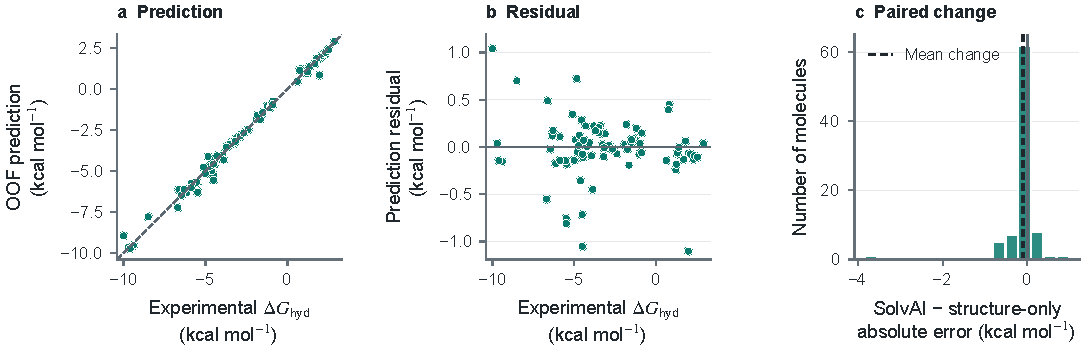
\includegraphics[width=\textwidth]{Supp_Fig1_residuals.pdf}
\end{center}
\noindent\textbf{Supplementary Figure 1 | Molecule-level prediction and residuals.}
\textbf{a}, Confirmatory response-augmented ExtraTrees OOF prediction against experiment. \textbf{b}, Signed
residual (prediction minus experiment) against experimental hydration free energy.
\textbf{c}, Distribution of the paired absolute-error change, responses minus the
matched structure-only endpoint; negative values favor responses.

\vspace{1.2em}
\begin{center}
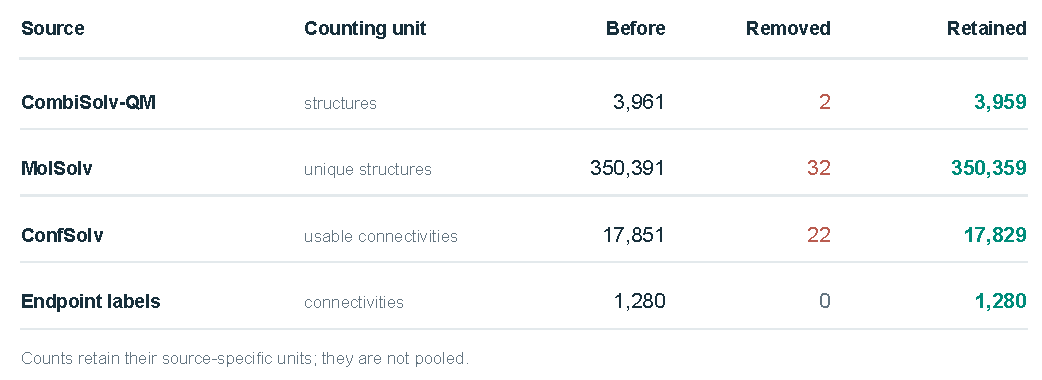
\includegraphics[width=\textwidth]{Supp_Fig2_provenance.pdf}
\end{center}
\noindent\textbf{Supplementary Figure 2 | Source-specific provenance and standardized
identity exclusion.} Counts before exclusion, removed counts and retained counts
are shown in their native source units. The audit removed standardized benchmark equivalents before the
confirmatory surrogate refits; no endpoint experimental label was removed.

\clearpage
\begin{center}
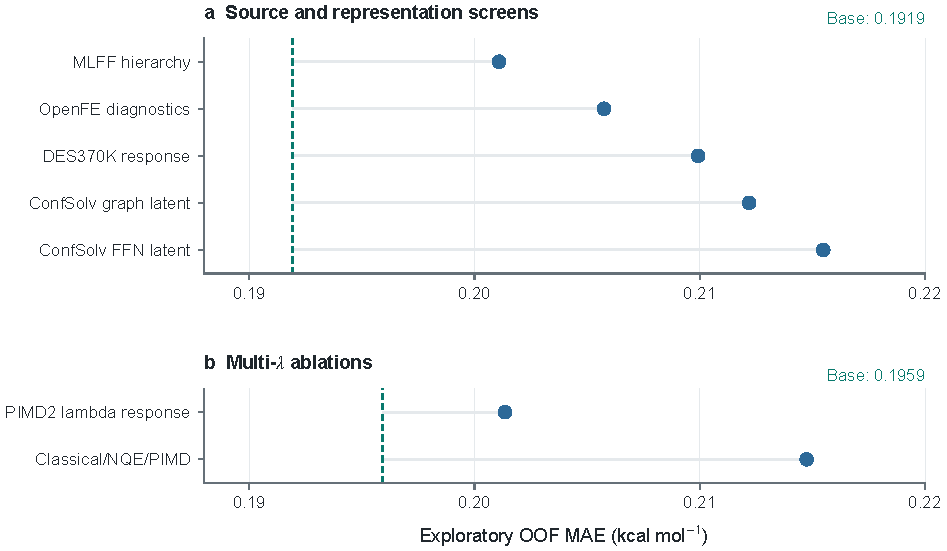
\includegraphics[width=0.88\textwidth]{Supp_Fig3_alternatives.pdf}
\end{center}
\noindent\textbf{Supplementary Figure 3 | Alternative physical-supervision routes.}
Exploratory fixed screens of additional diagnostic, latent and hierarchy features.
\textbf{a}, Source and representation screens use a one-seed SMD(water) plus ConfSolv
development base (0.1919 kcal mol$^{-1}$), whereas the final 15-coordinate
result averages three seeded fits. \textbf{b}, Multi-$\lambda$ ablations use
a separate fixed SMD(water) plus ConfSolv baseline (0.1959 kcal mol$^{-1}$).
Each dashed line marks the
corresponding control; gray segments connect that control to each screened
alternative. These experiments were not used to select the confirmatory controls.
OpenFE denotes the Open Free Energy toolkit; MLFF denotes machine-learning force
field; DES370K denotes the roughly 370,000-geometry intermolecular-interaction
dataset; FFN denotes feed-forward network.

\vspace{1.2em}
\begin{center}
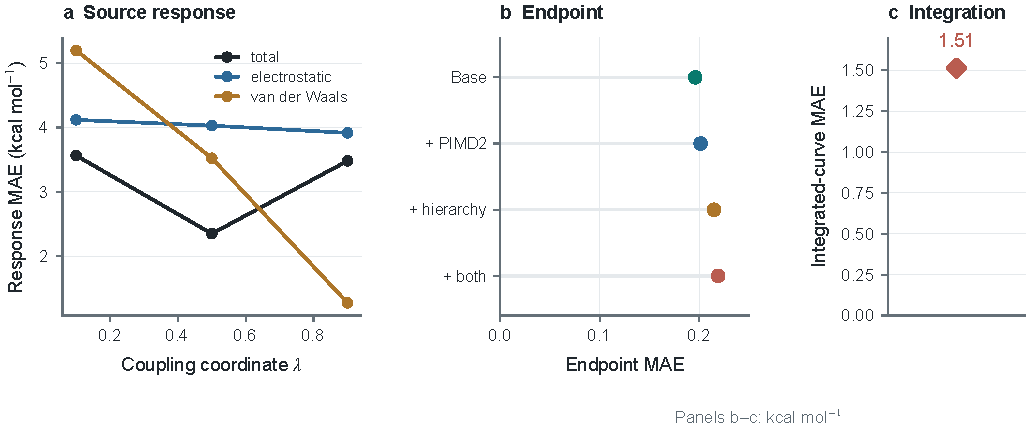
\includegraphics[width=\textwidth]{Supp_Fig4_lambda_response.pdf}
\end{center}
\noindent\textbf{Supplementary Figure 4 | Multi-$\lambda$ response experiment.}
\textbf{a}, OOF response-head error at three coupling states. \textbf{b}, Matched
endpoint consequences. \textbf{c}, Separately scaled error obtained by direct
integration of the predicted curve with fold-local affine calibration (diamond).

\clearpage
\begin{center}
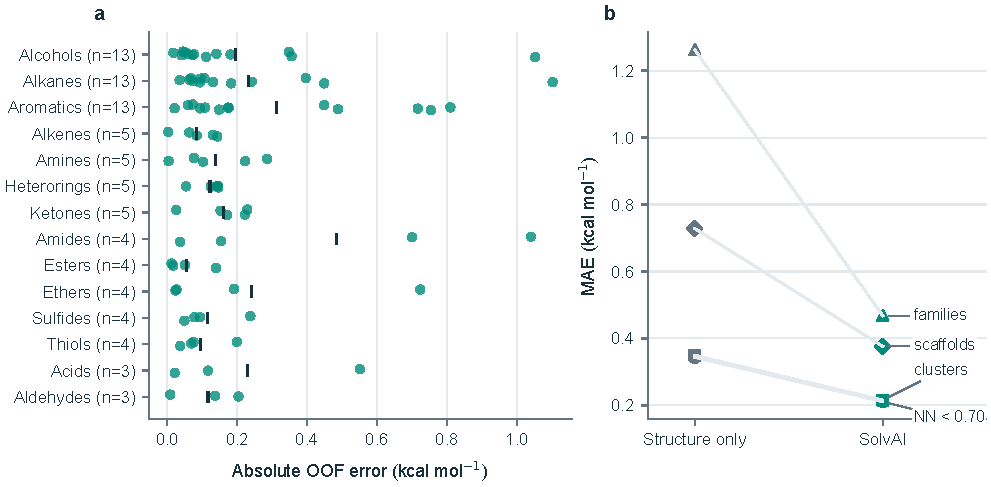
\includegraphics[width=\textwidth]{Supp_Fig5_extrapolation.pdf}
\end{center}
\noindent\textbf{Supplementary Figure 5 | Molecular errors by chemical family.}
Individual fixed-partition response-augmented ExtraTrees errors are grouped by diagnostic chemical
family; ticks show family means and labels give sample sizes. Global separation
results are shown in Fig.~\ref{M-fig:transfer}a,b.

\clearpage
\begin{center}
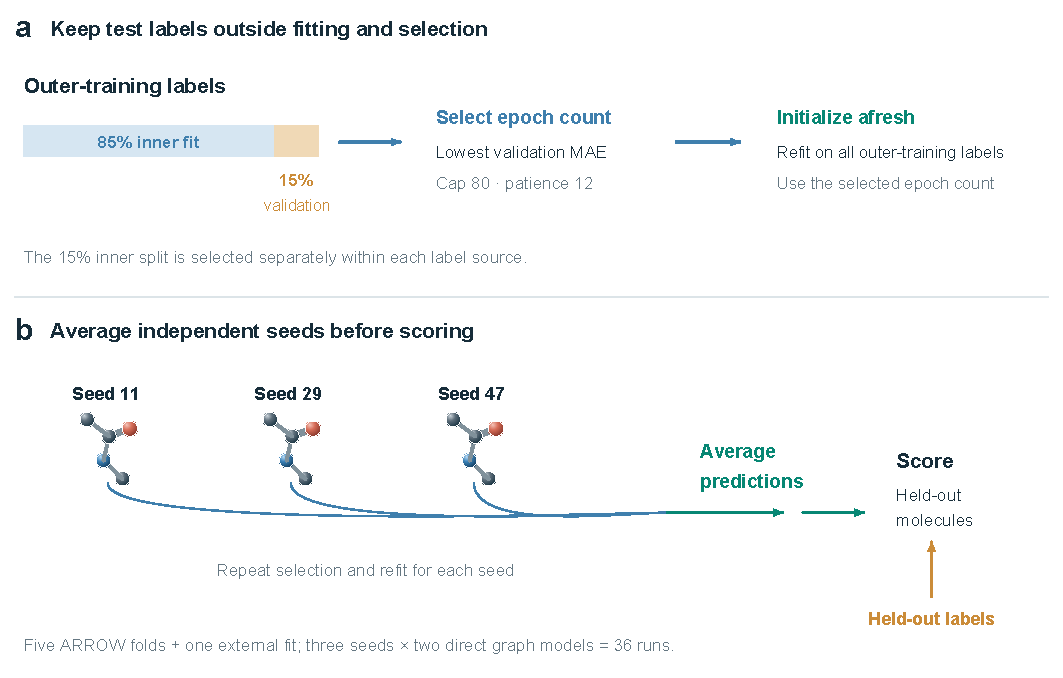
\includegraphics[width=\textwidth]{Supp_Fig6_evaluation_protocol.pdf}
\end{center}
\noindent\textbf{Supplementary Figure 6 | Select graph-model duration without using
held-out labels.} \textbf{a}, Within each outer-training set and seed, a deterministic
15\% of each label source is reserved for inner validation. The epoch with the lowest
unweighted validation MAE is selected, subject to an 80-epoch cap and patience 12.
A model reinitialized from its original random or CheMeleon starting weights is
then refitted on all outer-training labels for that
many epochs, with a newly fitted training scaler. \textbf{b}, Selection and refitting
are repeated for seeds 11, 29 and 47. Their predictions are averaged before comparison
with held-out labels. The five ARROW folds and one all-training external fit give
36 seed-level runs across the scratch D-MPNN and fine-tuned CheMeleon models. The
colored vectors represent predictions for held-out molecules, not new training inputs.

\clearpage
\begin{center}
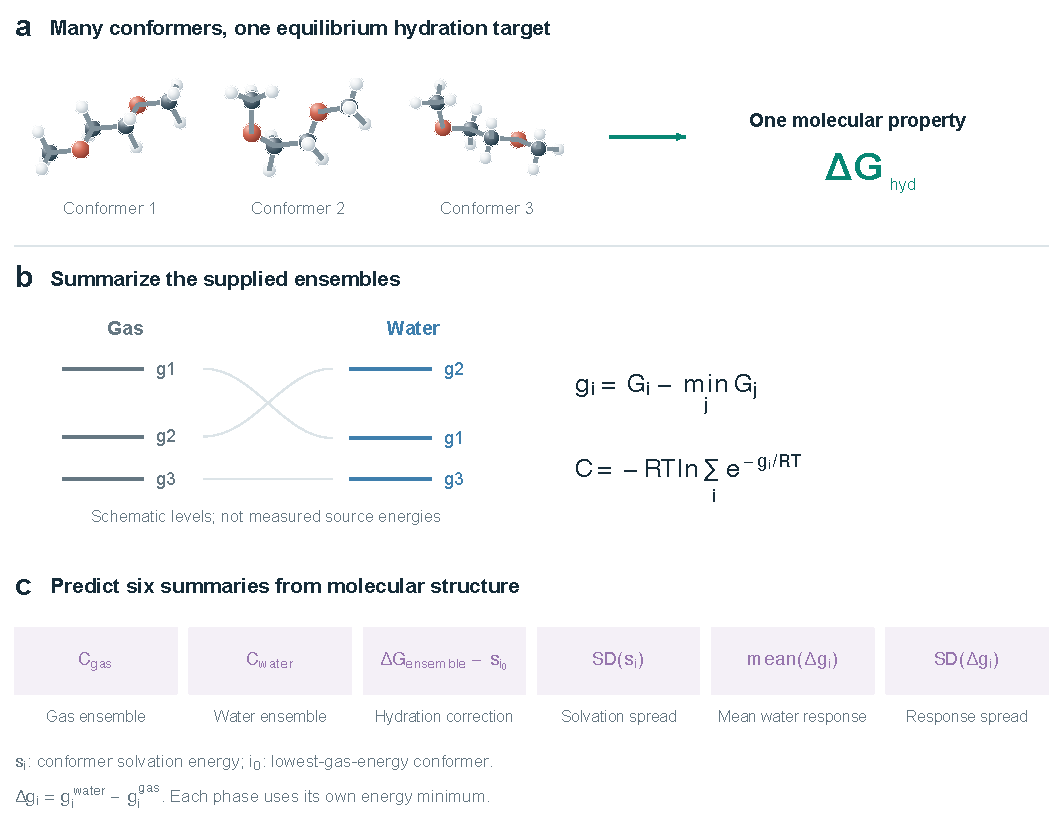
\includegraphics[width=\textwidth]{Supp_Fig7_conformer_targets.pdf}
\end{center}
\noindent\textbf{Supplementary Figure 7 | Conformer-resolved sources teach a molecular
equilibrium response.} \textbf{a}, Three illustrative conformers of
1,2-dimethoxyethane share one molecular equilibrium hydration target; they do not have
separate experimental endpoint labels. \textbf{b}, Gas and water conformer energies
are normalized separately to their phase-specific minima, giving $g_i$. The
correction $C=-RT\ln\sum_i\exp(-g_i/RT)$ summarizes the supplied ensemble. Energy
levels and their connecting lines are schematic, not measured ConfSolv energies.
\textbf{c}, The six predicted summaries are the gas and water corrections, ensemble
hydration minus the solvation energy of the lowest-gas-energy conformer, the population
standard deviation of conformer solvation energies, and the arithmetic mean and
population standard deviation of $\Delta g_i$. All energies are in kcal mol$^{-1}$.
These summaries do not assert complete conformational sampling, and no conformer
ensemble is regenerated at deployment.

\clearpage
\begin{center}
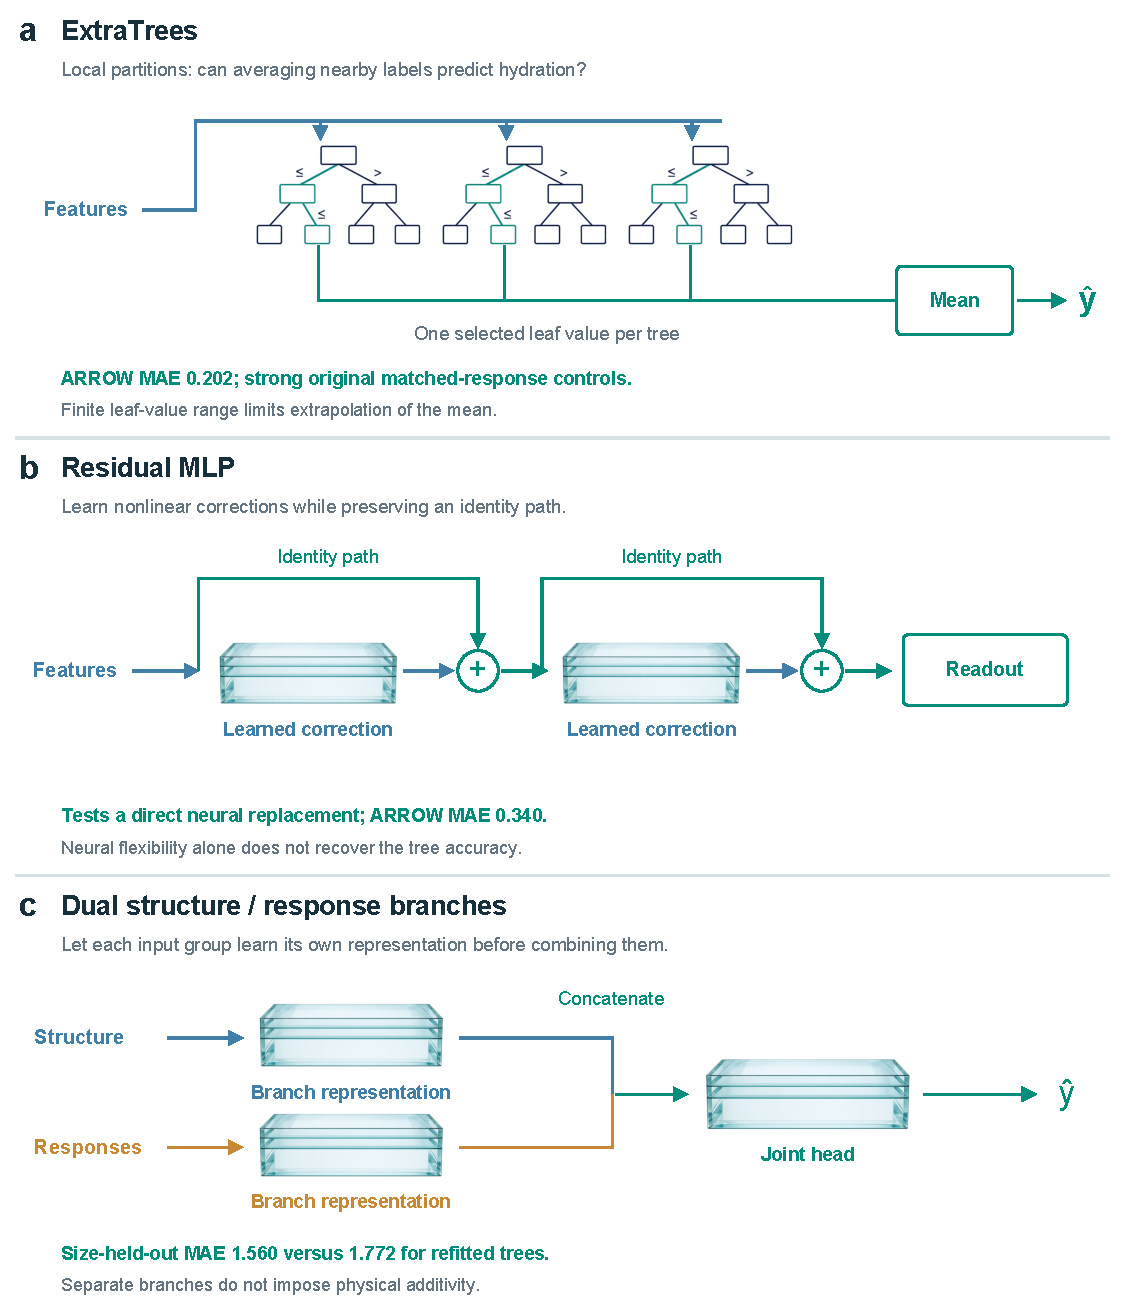
\includegraphics[width=\textwidth]{Supp_Fig8_endpoint_mechanisms.pdf}
\end{center}
\noindent\textbf{Supplementary Figure 8 | Local averaging and neural feature combination.}
\textbf{a}, ExtraTrees selects a leaf in each randomized tree and averages its
stored value. \textbf{b}, A residual MLP learns corrections alongside identity
paths. \textbf{c}, Separate structural and response branches are concatenated
before a joint head. Illustrations explain mechanisms, not exact layer widths or
tree counts. Numerical callouts refer to the evaluations in Table~2, not theoretical
properties of the architectures. All mechanism diagrams use editable vector
geometry; they are explanatory schematics, not data-derived plots.

\clearpage
\begin{center}
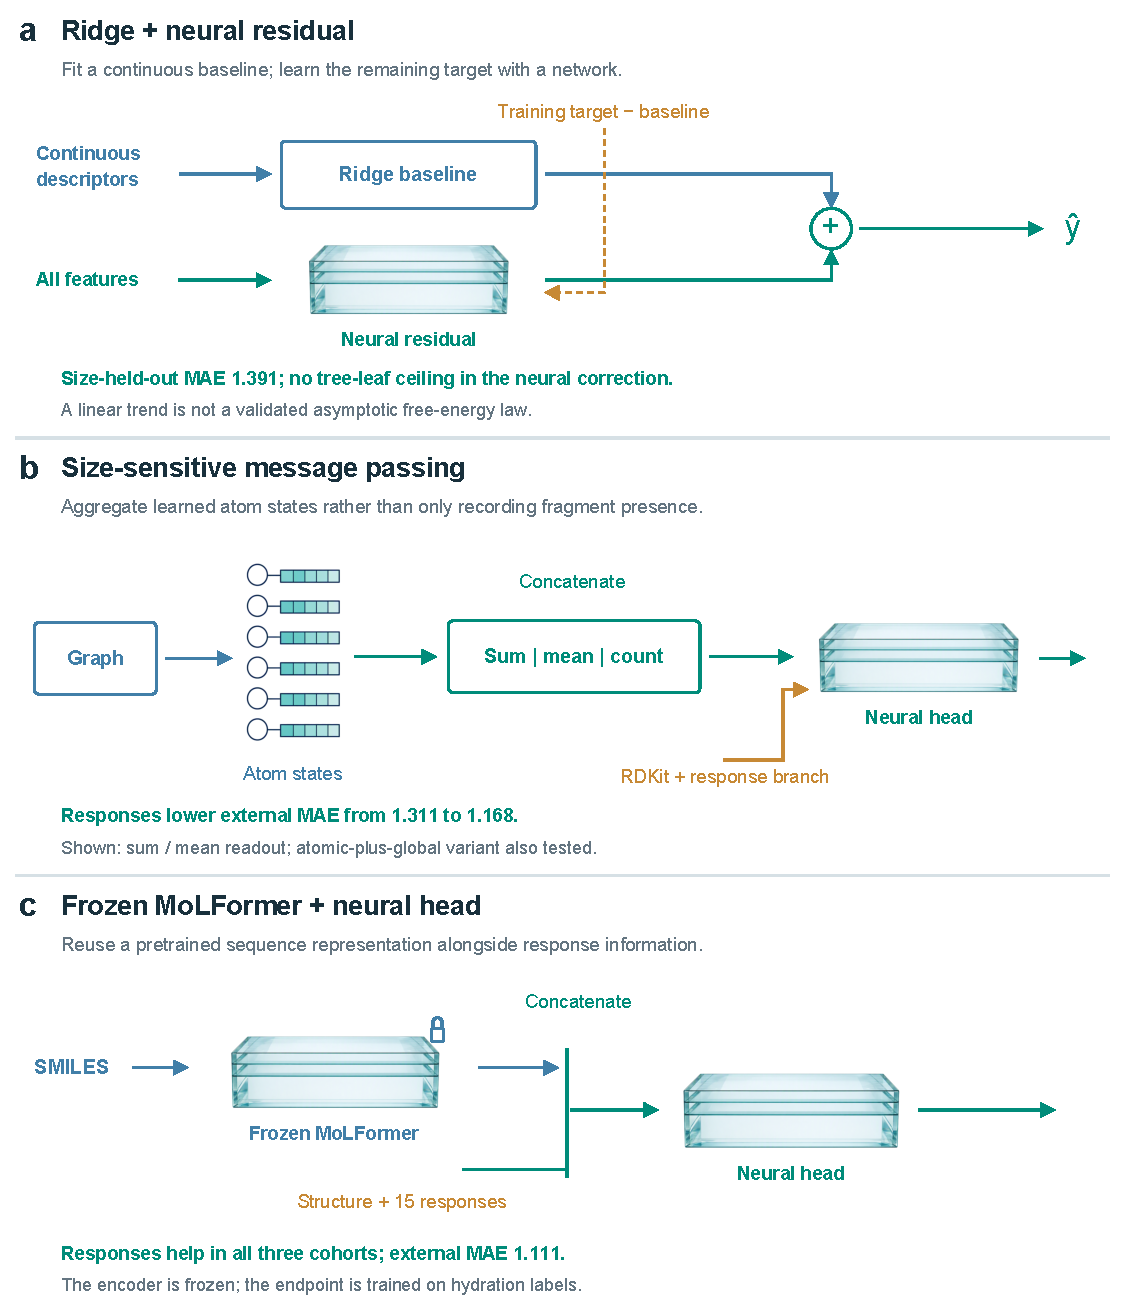
\includegraphics[width=\textwidth]{Supp_Fig9_endpoint_mechanisms.pdf}
\end{center}
\noindent\textbf{Supplementary Figure 9 | Baselines, graph aggregation and pretrained encodings.}
\textbf{a}, Ridge predicts a continuous baseline and a network learns the remaining
target, $y-b(x)$, during training; inference adds the baseline and predicted residual
without access to the query's target. \textbf{b}, One graph variant combines summed and mean atom states
with atom-count information; a separate atomic-plus-global variant is also tested.
The summaries are concatenated, not numerically equated or treated as independent
free-energy contributions. \textbf{c}, MoLFormer is frozen, while the downstream
head learns to combine its representation with structural and response information.
Schematics omit layer detail; all source surrogates remain fixed.

\clearpage
\begin{center}
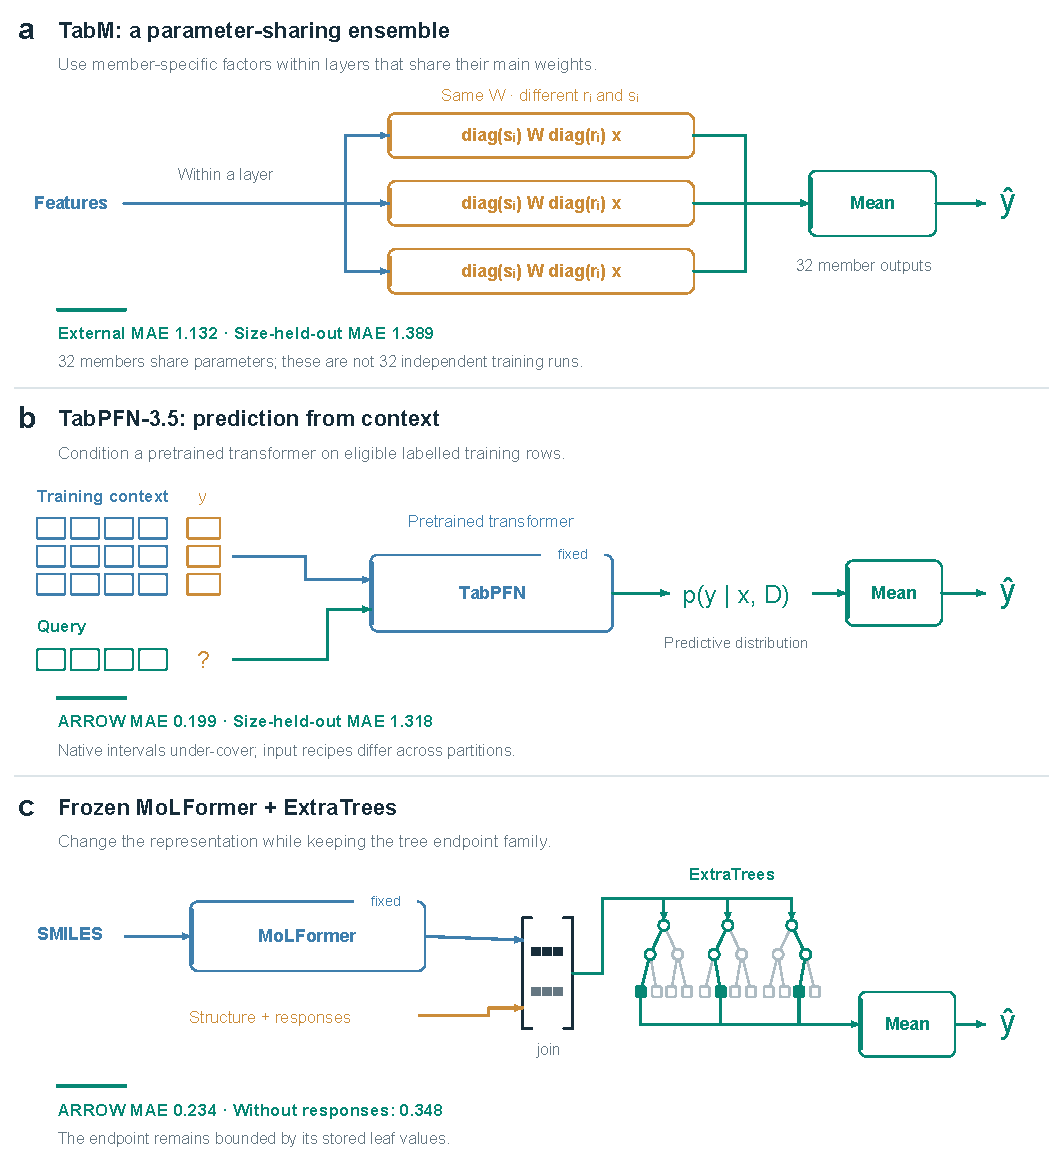
\includegraphics[width=\textwidth]{Supp_Fig10_endpoint_mechanisms.pdf}
\end{center}
\noindent\textbf{Supplementary Figure 10 | Shared ensembles, in-context inference and a representation control.}
\textbf{a}, TabM shares weight matrices while member-specific input/output
modulations within its layers produce 32 predictions. Three paths are shown for
clarity; the mean is used. \textbf{b}, TabPFN conditions on labelled training rows
and an unlabelled query using pretrained weights. No query label is supplied and
no gradient fine-tuning is done here. Feature recipes vary by partition (S19).
\textbf{c}, Frozen MoLFormer features are combined with structural and response
features before an ExtraTrees endpoint, isolating a representation change while
retaining leaf-value averaging. Three representative trees are shown, not the full ensemble.

\clearpage
\begin{center}
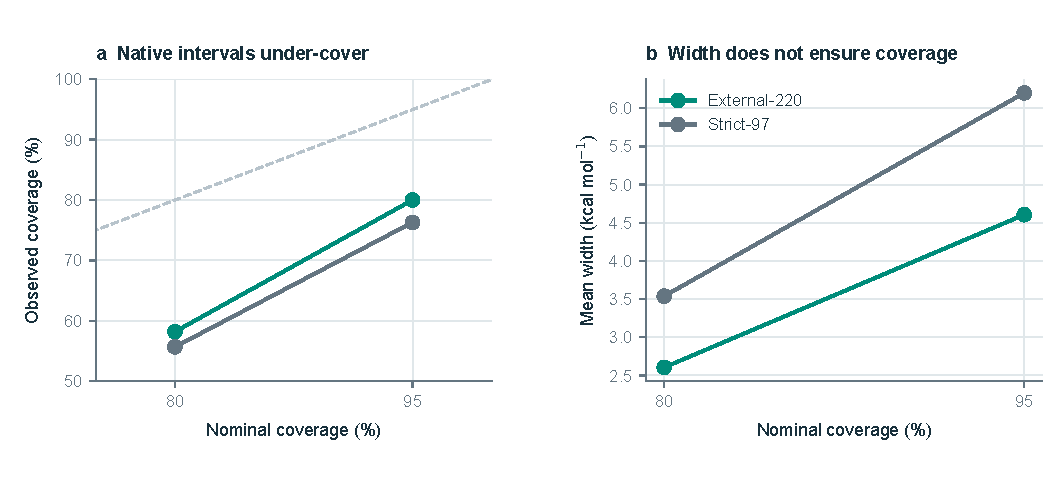
\includegraphics[width=\textwidth]{Supp_Fig11_uncertainty.pdf}
\end{center}
\noindent\textbf{Supplementary Figure 11 | Native predictive intervals require calibration.}
\textbf{a}, Empirical versus nominal coverage for the equal five-model TabPFN
mixture; the dashed diagonal marks nominal coverage. \textbf{b}, Corresponding
mean interval widths. Strict-97 is nested in External-220. These intervals are
shown in teal for External-220 and gray for Strict-97 in both panels. They are
evaluated without external calibration, and their undercoverage is not represented
by seed dispersion. Connecting lines guide the eye between the two assessed levels.

\clearpage
\begin{center}
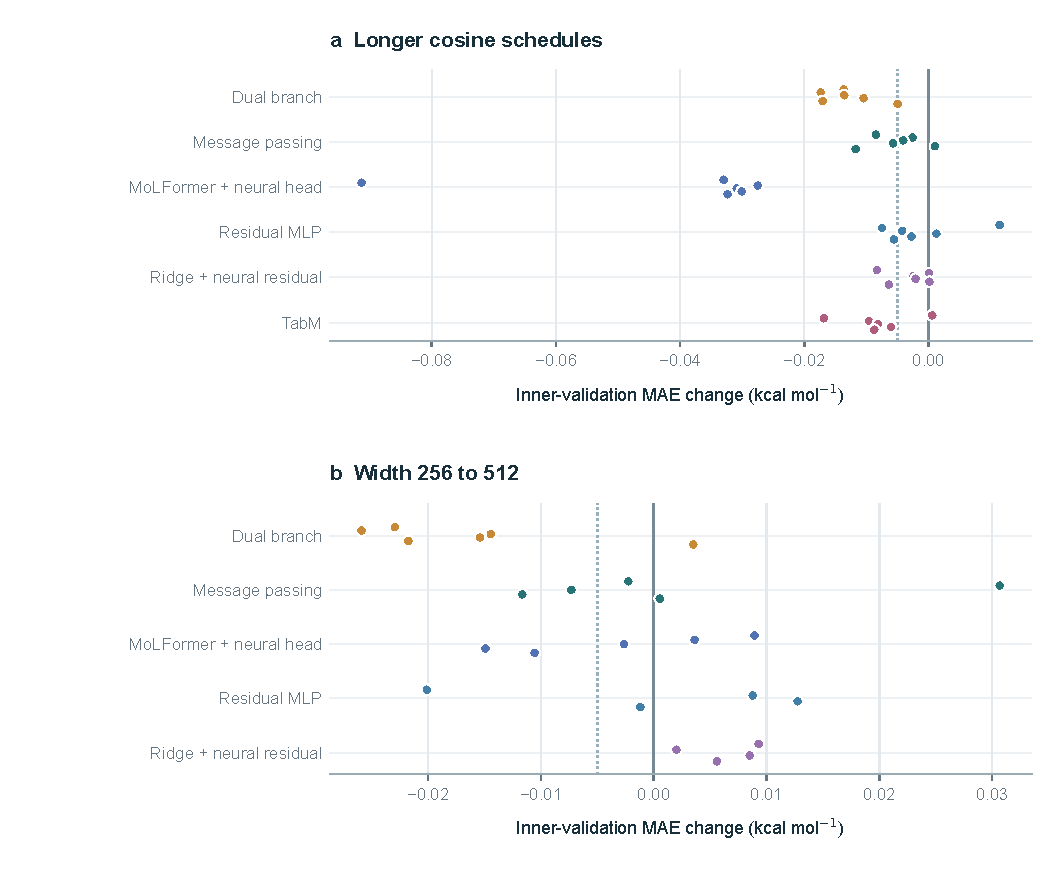
\includegraphics[width=\textwidth]{Supp_Fig12_optimization.pdf}
\end{center}
\noindent\textbf{Supplementary Figure 12 | Training duration and capacity challenges.}
\textbf{a}, Mean three-split inner-validation changes at seed 47 for the
1,200-epoch cosine challenge relative to the ordinary schedule, one dot per outer
partition and family. \textbf{b}, Corresponding changes when width is expanded
from 256 to 512 for qualifying configurations. Negative favors the challenge;
the dotted line marks $-0.005$ kcal mol$^{-1}$. Retention also requires improvement
in at least two of the three pairs. These are inner-validation scores, not test
results, and the duration challenge also changes the learning-rate schedule.

\bibliographystyle{unsrtnat}
\bibliography{references}
\end{document}
